\chapter{绪论}\label{chap:kondo}

\section{冷原子概述}

杂质物理,其中少体体系与多体体系

%\subsection{冷原子基本实验技术}

冷却囚禁费米子技术

光晶格

Feshbach resonance

Confiment induced resonance

\section{费米子少体体系}\label{sec:fewbody}
伴随着冷原子平台实验技术的进步,各个凝聚态研究领域掀起了不同程度的热潮。其中少体物理的研究领域有了较大进展。得益于实验中少量原子体系的
制备、调控与测量,少体物理中很多概念诸如少体束缚态、费米化等理论概念不断地在冷原子实验中被观测到,并进而引发了冷原子特性平台下相关少体物理的理论研究。实际的冷原子少体体系中几个原子被束缚在势阱中,因此我们的内容也主要限制在束缚势阱中的少体体系实验与理论研究进展,以期为接下来的研究提供启发,更细致全面的review可推荐\cite{sowinski2019one,blume2012few},本章还不会涉及Efimov物理,相关review参见\cite{nielsen2001three,braaten2006universality,KohlerMolFRRMP}。由于原子间全同性原理,我们将围绕玻色少体体系与费米少体体系分别展开。束缚的原子数可控程度越来越高,体系的维度可以通过各向异性的势阱实现,原子之间的相互作用均可以调节,从极弱到极强,从吸引到排斥。进一步选取不同的混合体系带来质量比的可调节性,这些丰富的可调节实验条件为少体体系带来丰富的物理。

\subsection{费米少体实验}
实验中最早制备出费米子少体体系可以追溯到2005年,在较深的光晶格体系中,进入到莫特绝缘体区域,制备少体体系\cite{greiner2002quantum,EsslingerFermiSea,Esslinger1DMol,Esslinger3DMol,Ospelkaus3DMol,Hecker3DMol,SalaCIRMol}。如图~\ref{3dmol}~所示,
\begin{figure}[!htbp]
    \centering
    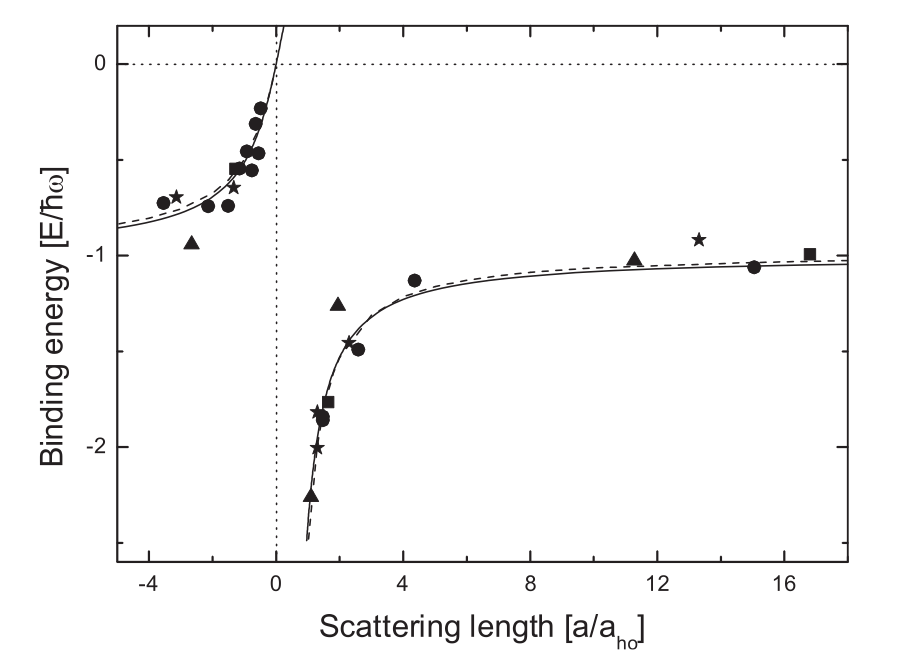
\includegraphics[width=0.5\textwidth]{chap13dmol.png}
    \bicaption{三维光晶格中的Feshbach分子态。散点代表不同晶格深度的实验数据。实线代表理论数据。摘自 \cite{Esslinger3DMol}}{The measured binding energy of molecules in a 3D optical lattice. Scatterd points for defferent depth of latice. The solid line for theory. Reprinted from \cite{Esslinger3DMol}}
    \label{3dmol}
\end{figure}
实验观测到了较深光晶格内调节磁场形成的Feshbach分子态。
但是沿着另外一个思路,精确制备少体体系\cite{SerwaneDeterministic,zurn2012fermionization,WenzFermiSeaOnebyOne,Zurn2013Pairing,MurmannSpinChain,MurmannTwoFermionDoubleWell,RontaniTunneling}。

首先,Serwanel实现了一种可以确定性制备不同原子数目的手段,通过能级间距较大的microtrap与两分量${}^6$Li原子热库接触到的热平衡,制备$T/T_F\sim0.08$含有600多个原子的费米球,费米面最低能级的原子占据数可达0.9999。然后在microtrap上施加磁场梯度,使得trap一端势能降低,从而原子可以漏出。然后绝热地改变microtrap的深度,便可使得原子不断漏出,最终达到只含有几个原子的微小体系。如图~\ref{deter}~所示。
\begin{figure}[!htbp]
    \centering
    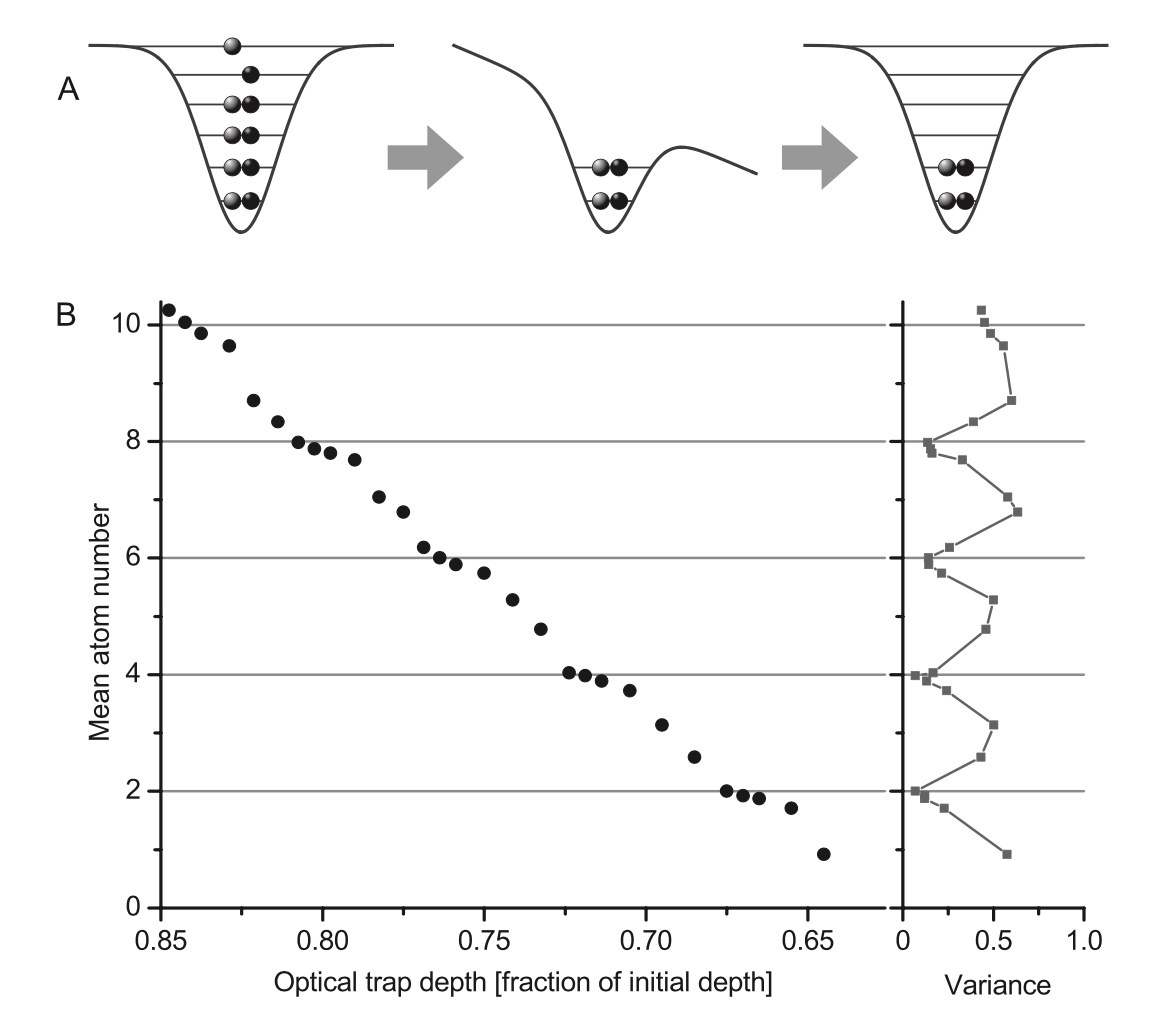
\includegraphics[width=0.5\textwidth]{chap1deter.png}
    \bicaption{图A表示降低深度使原子漏出来制备少体的示意图。图B为实验测到的少体体系平均粒子数与方差。 摘自 \cite{SerwaneDeterministic} }{FIG. 2 (A) for illustration of spilling. Fig (B) for measured mean density and variance. Reprinted from\cite{SerwaneDeterministic} }
    \label{deter}
\end{figure}

然后,借助上面精确制备少体体系的方法,研究者研究了不同自旋费米子$\uparrow\downarrow$之间费米化的过程。在准一维trap中制备两体少体体系,调节不同自旋费米子之间的相互作用。通过少体体系隧穿几率反应两体的能量。最终得到隧穿几率如图~\ref{ferminization}~
\begin{figure}[!htbp]
    \centering
    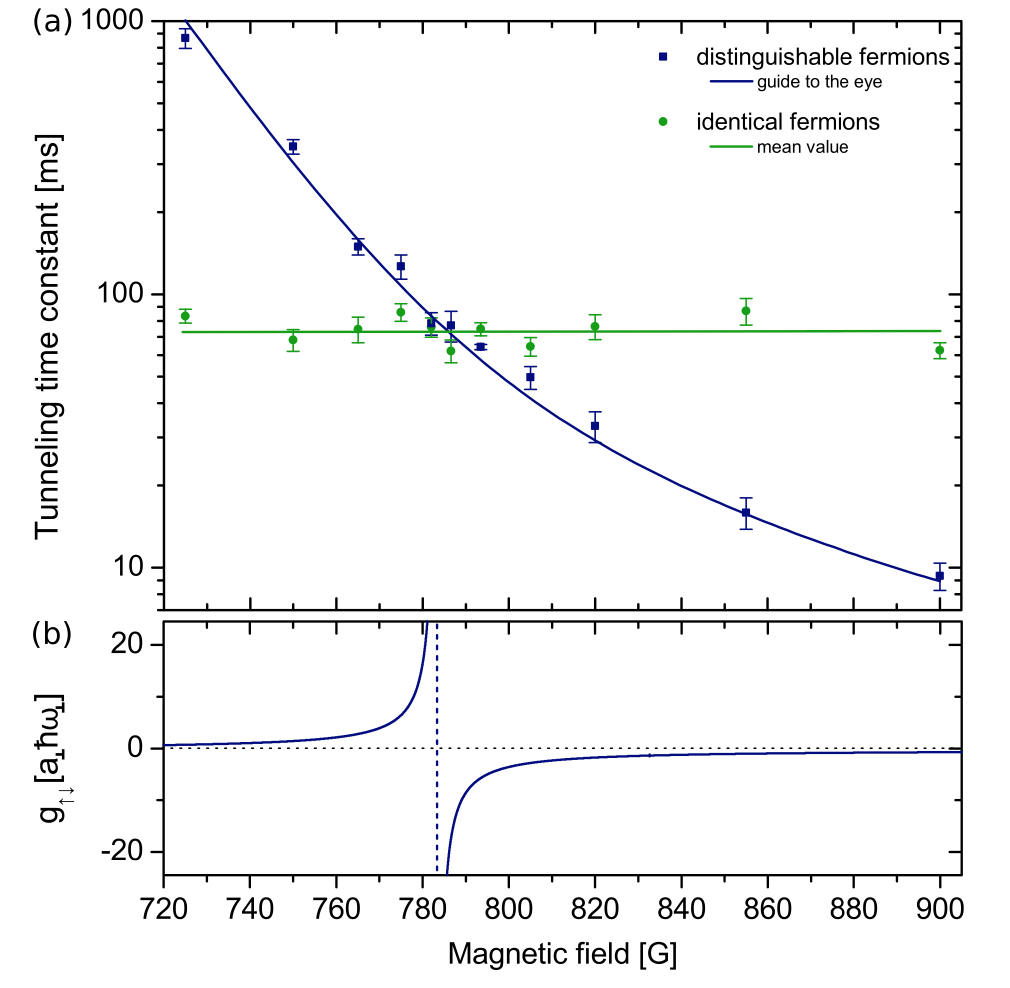
\includegraphics[width=0.5\textwidth]{chap1ferminization.png}
    \bicaption{不同的有效一维相互作用下两体费米子隧穿几率。谐振子势阱中两体体系的能量决定了隧穿几率。其中在共振点处相互作用费米子$\uparrow\downarrow$能量等于无相互作用全同费米子$\uparrow\uparrow$能量,发生费米化。 摘自 \cite{zurn2012fermionization} }{Tunneling time constant for different 1D effective interaction strengths. Two body energy decides the tunneling time constant. The same tunneling constant of $\uparrow\downarrow$ at resonance point as $\uparrow\uparrow$ reflects the ferminization. Reprinted from\cite{zurn2012fermionization} }
    \label{ferminization}
\end{figure}
所示,同自旋费米子之间无相互作用,调节磁场后两体能级没有变化。但是不同费米子之间相互作用在共振点处发散,对应能量与无相互作用费米子能量相同,体系发生费米化。


进一步地,研究从少体到多体的过渡。基本模型是谐振子势阱下N+1的一维极化子物理。相互作用只存在于少数原子与多数原子之间,并且可以通过Feshbach共振调节。从1到5增加多数原子的数目,用rf脉冲测量不同相互作用下极化子的能量,通过与理论计算的1+1与1+$\infty$体系的能量密度进行比较,可以发现在粒子数为5的时候能量上就很接近多体体系了。如图~\ref{fermisea}~所示。
\begin{figure}[!htbp]
    \centering
    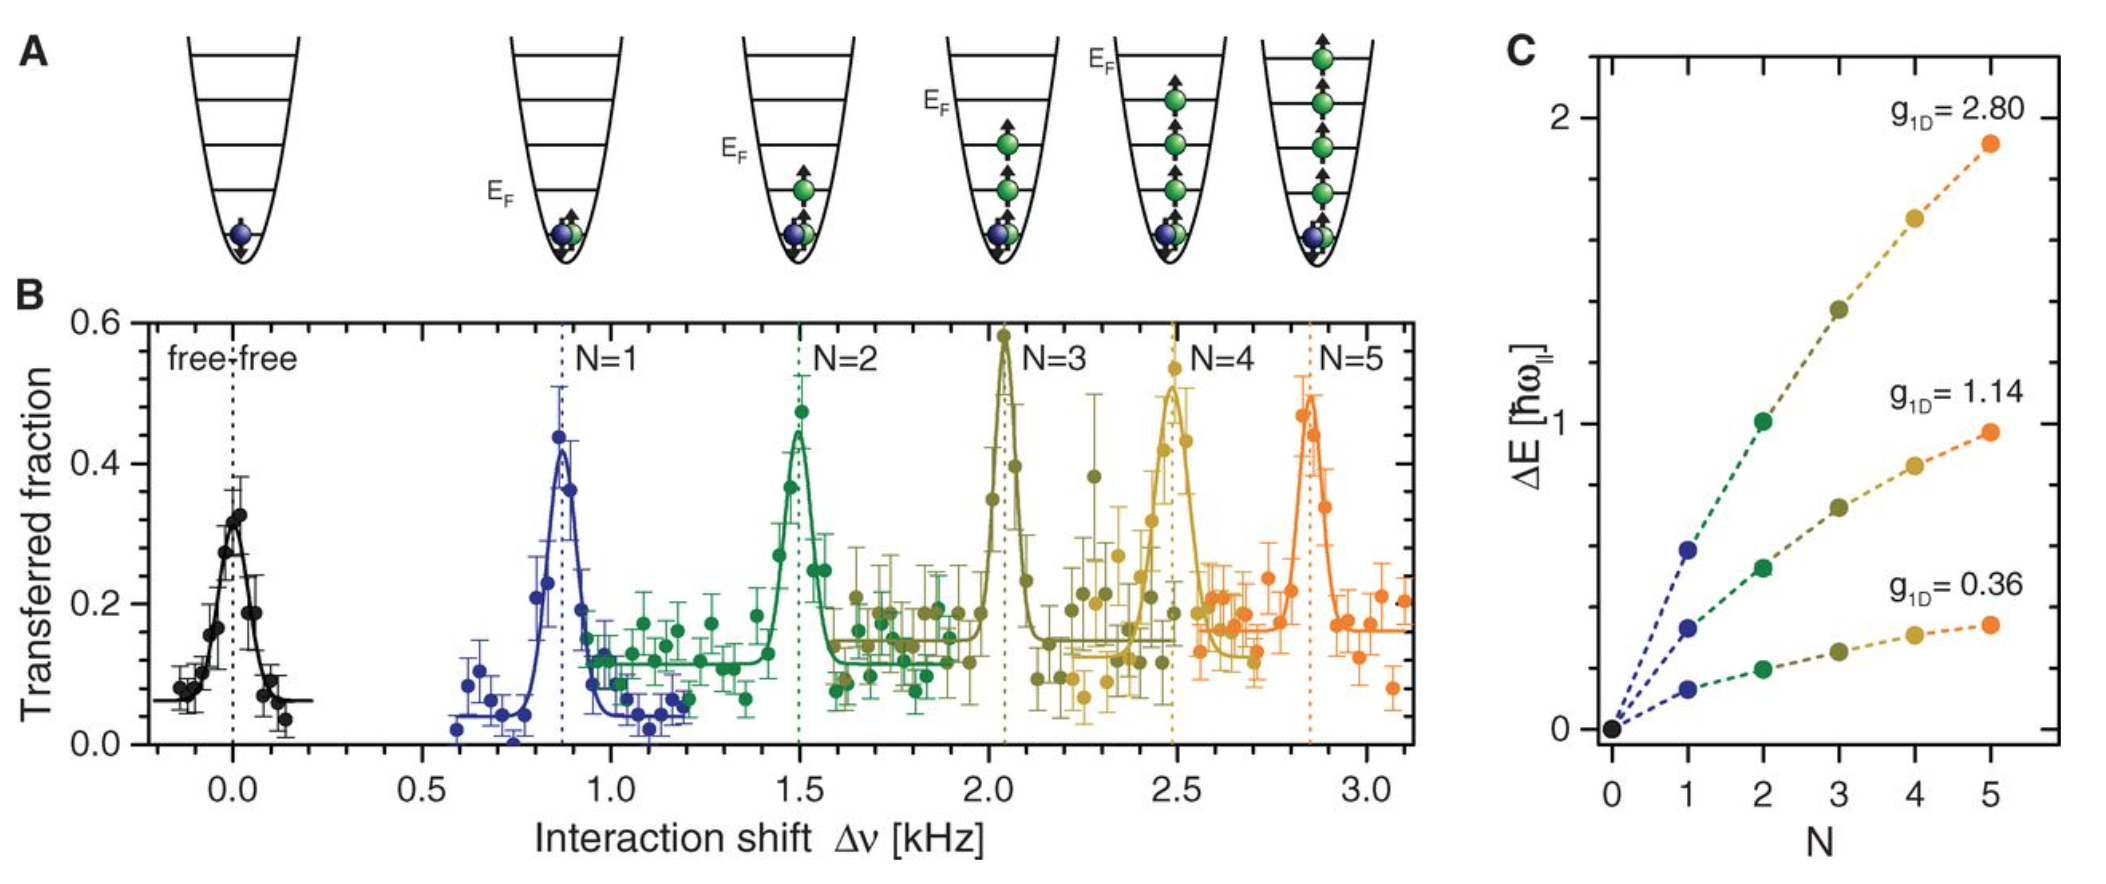
\includegraphics[width=0.8\textwidth]{chap1fermisea.png}
    \bicaption{ 图A为谐振子势阱中1+N体系能谱示意图。图B为实验测得的rf脉冲谱。图C为能量密度。摘自 \cite{WenzFermiSeaOnebyOne} }{Fig (A) for energy spectrum of 1+N system. Fig (B) for measured rf spectrum. Fig (C) for energy difference. Reprinted from\cite{WenzFermiSeaOnebyOne} }
    \label{fermisea}
\end{figure}

不仅通过能量角度,进一步从关联的角度,少体体系性质也得以研究。通过制备$(N_\uparrow,N_\downarrow)=(2,1,(3,1),(2,2)$少体体系,绝热地调节不同自旋之间相互作用从自由极限到Tonks极限,越过共振点进入super Tonks极限,制备了反铁磁自旋连与铁磁自旋链。
\begin{figure}[!htbp]
    \centering
    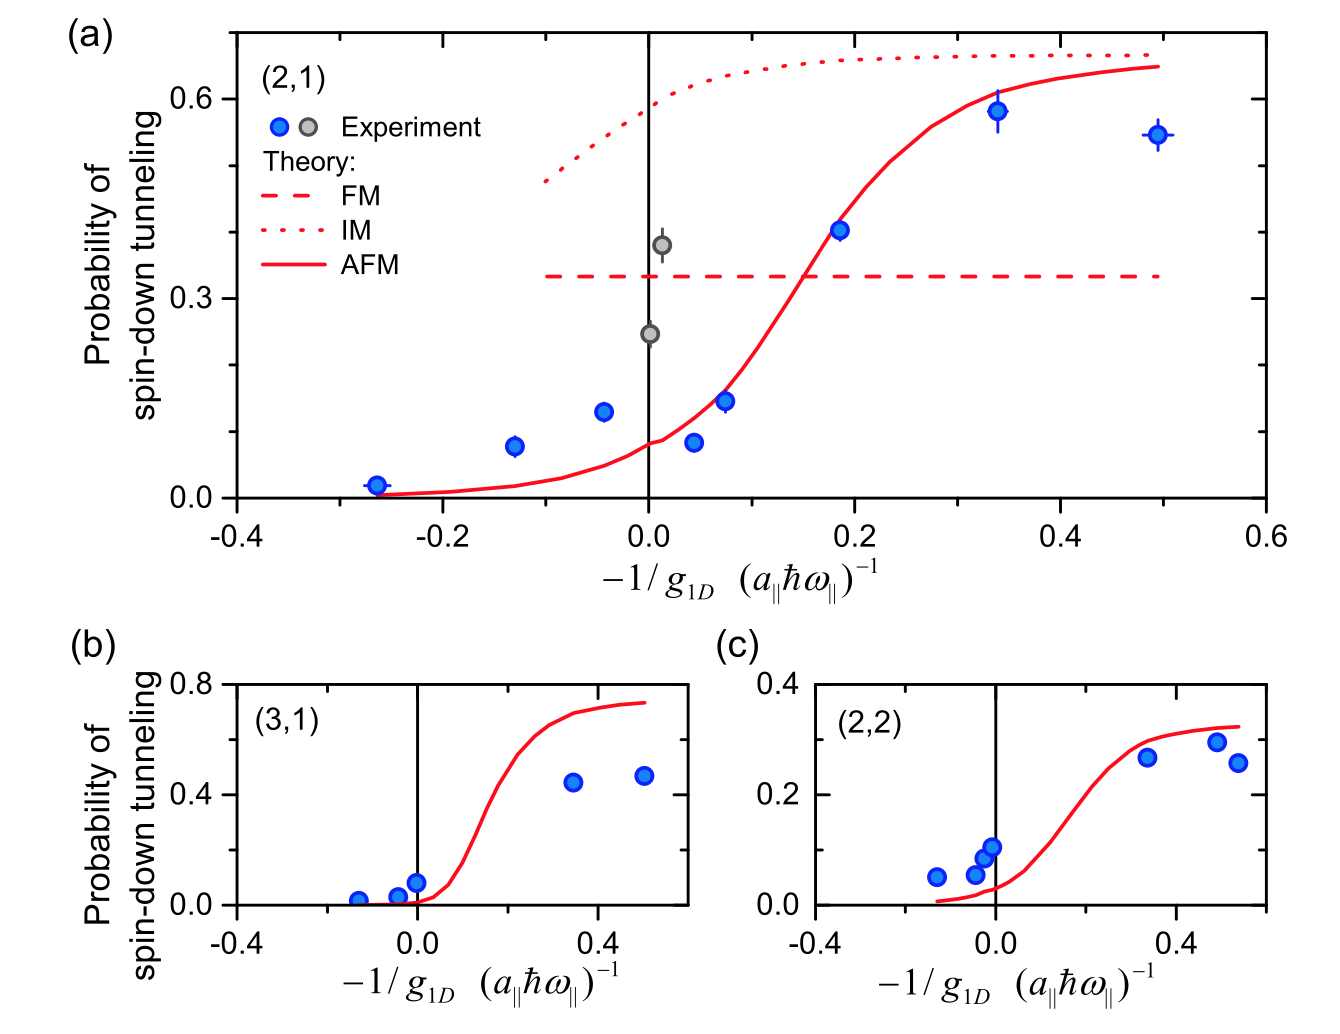
\includegraphics[width=0.7\textwidth]{chap1spinchain.png}
    \bicaption{ 不同少体体系$\downarrow$原子隧穿几率随一维有效相互作用的变化,a为(2,1),b为(3,1),c为(2,2)。散点为实验测得数据。线条代表不同的自旋链模型计算得到的隧穿几率。摘自 \cite{MurmannSpinChain} }{Tunneling rate of $\downarrow$ atom in different few body systems upon 1D effective coupling constant. a for (2,1), b for (3,1) and cc for (2,2). Reprinted from\cite{MurmannSpinChain} }
    \label{chap1spinchainexp}
\end{figure}
实验上通过让边缘处的粒子漏出,来测量自旋分布。漏出的几率由初态能量与末态能量决定。通过与理论自旋链模型的漏出几率对比,可以确认制备到反铁磁自旋链。如图~\ref{chap1spinchainexp}~所示。


\subsection{费米少体理论}
少体物理之所以重要是因为可以提供一个可理解的物理图像,甚至某些特殊体系存在严格解。这些少体图像成了我们理解实验的基石。在冷原子领域,有两个经典的两体图像,分别是:自由空间s波散射图像与谐振子势场下s波相互作用两体严格解。由于本节内容关在存在外势的相关少体物理,因此我们从介绍后者出发。

1998年T. Busch给出了又一个少体体系严格解:任意维度下两个全同玻色子在谐振子势场下的能谱。虽然是玻色子体系,但是这个严格解同样适用于可分辨费米子。三维情况下,可分辨两体全同费米子位于谐振子外势下,系统的哈密顿量可以写为:
\begin{equation}
\hat{H}=-\frac{1}{2} \nabla_{1}^{2}-\frac{1}{2} \nabla_{2}^{2}+\frac{1}{2} r_{1}^{2}+\frac{1}{2} r_{2}^{2}+4 \pi a_{0} \delta_{r e g}^{(3)}\left(\Vector{r}_{1}-\Vector{r}_{2}\right)
\end{equation}
能量量纲为$\hbar\omega$,长度量纲为$\sqrt{\hbar}{m\omega}$,$a_0$代表散射长度。其中$m$为全同玻色子的质量,$\omega$为谐振子势场的特征频率。分离质心运动$\Vector{R}=\sqrt{1 / 2}\left(\Vector{r}_{1}+\Vector{r}_{2}\right)$与相对运动$\Vector{r}=\sqrt{1 / 2}\left(\Vector{r}_{1}-\Vector{r}_{2}\right)$
得到:
\begin{equation}
\begin{aligned}
&H_{\mathrm{CM}}=-\frac{1}{2} \nabla_{R}^{2}+\frac{1}{2} \mathbf{R}^{2}\\
&H_{r e l}=-\frac{1}{2} \nabla_{r}^{2}+\frac{1}{2} \mathbf{r}^{2}+\sqrt{2} \pi a_{0} \delta^{(3)}(\mathbf{r}) \frac{\partial}{\partial r} r\\
\end{aligned}
\end{equation}
质心运动的部分是自由谐振子。只剩相对运动部分,满足的薛定谔方程为:
\begin{equation}
\left(H_{o s c}+\sqrt{2} \pi a_{0} \delta^{(3)}(\mathbf{r}) \frac{\partial}{\partial r} r\right) \Psi(\mathbf{r})=E \Psi(\mathbf{r})
\end{equation}
相对运动部分的$l\neq=0$空间不受相互作用影响,仍为自由谐振子,只考虑$l=0$子空间。波函数展开在谐振子基矢下:
相应的本征波函数为:
\begin{equation}
\Psi(\mathbf{r})=\sum_{n=0}^{\infty} c_{n} \varphi_{n}(\mathbf{r})
\end{equation}
带入到薛定谔方程里得到:
\begin{equation}
c_{n}\left(E_{n}-E\right)+\sqrt{2} \pi a_{0} \varphi_{n}^{*}(0)\left[\frac{\partial}{\partial r}\left(r \sum_{m=0}^{\infty} c_{m} \varphi_{m}(\mathbf{r})\right)\right]_{r \rightarrow 0}=0
\end{equation}
求得$c_n$满足:
\begin{equation}
c_{n}=A \frac{\varphi_{n}^{*}(0)}{E_{n}-E}
\end{equation}
将系数带回到薛定谔方程得到本征能量满足:
\begin{equation}
\sqrt{2} \frac{\Gamma(-E / 2+3 / 4)}{\Gamma(-E / 2+1 / 4)}=\frac{1}{a_{0}}
\end{equation}
对应的本征波函数解析形式为:
\begin{equation}
\Psi(\mathbf{r})=\frac{1}{2} \pi^{-3} / 2 A e^{-r^{2} / 2} \Gamma(-v) U\left(-v, \frac{3}{2}, r^{2}\right)
\end{equation}
其能谱随着散射长度如图~\ref{chap1busch}~所示:
\begin{figure}[!htbp]
    \centering
    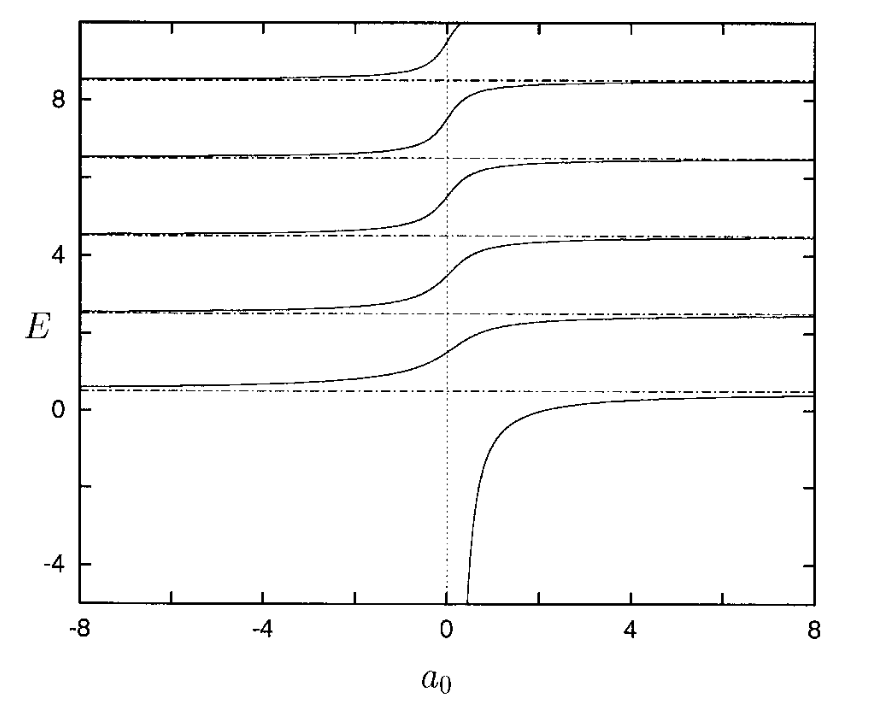
\includegraphics[width=0.6\textwidth]{chap1busch.png}
    \bicaption{摘自1D少体势阱}{Reprinted from 1Dfewtrap}
    \label{chap1busch}
\end{figure}
其中当$a_0\to \infty$时候,基态能量渐近行为是$E_g\propto - a_0^2$,称为lower branch。其余的随着$a_0\to\infty$本征能量饱和在奇数谐振子能量的态称为upper branch。这个少体体系的严格解在后续的实验与理论发展中起了很重要的做用。

自然地,一维以及二维的结果,也可用上述求解给出。其中一维的能量方程与三维相同,不同在于能量相对于偶宇称的解。二维下能量方程则有很大不同:
\begin{equation}
\psi(-E / 2+1 / 2)=\log \left(\frac{1}{2 a_{0}^{2}}\right)
\end{equation}

后续对这个体系的严格解有了一些扩展,主要是各项异性的谐振子外势求解,以及动力学研究\cite{blume2012few}。而对于再增加一个粒子成为三体体系则没有了解析解,只能通过数值手段去求解。

我们讨论$\uparrow\downarrow\uparrow$的费米子三体体系,仅在不同自旋费米子之间有s波散射相互作用\cite{OlshaniiRigorous2001,Petrov2003unitary3b,Fleix2006prlunitary3b,Felix2006praunitary3b,LmDuan2007levelcrossing,Stetcu2007,Blume2008,Blume2010,Xiaji2009prl,Xiaji20103b,Rittenhouse2010green}。我们用Bethe-Peierls条件代替:
\begin{equation}
\psi\left(\mathbf{r}_{1}, \mathbf{r}_{2}, \mathbf{r}_{3}\right)=\left(\frac{1}{r_{i j}}-\frac{1}{a}\right) A\left(\mathbf{R}_{i j}, \mathbf{r}_{k}\right)+O\left(r_{i j}\right)
\end{equation}
其中$r_{i j} \equiv\left|\mathbf{r}_{i}-\mathbf{r}_{j}\right| \rightarrow 0$,$\mathbf{R}_{ij}$为两原子的质心位置。

三维情况下这种体系的求解\cite{Fleix2006prlunitary3b}借助于HyperSphere框架,先引入Jacobi坐标:
\begin{equation}
\begin{split}
\Vector{r}&=\Vector{r}_{2}-\Vector{r}_{1}\\
\boldsymbol{\rho}&=\left(2 \mathbf{r}_{3}-\mathbf{r}_{1}-\mathbf{r}_{2}\right) / \sqrt{3}\\
\Vector{C}&=\left(\Vector{r}_{1}+\Vector{r}_{2}+\Vector{r}_{3}\right) / 3\\
\end{split}
\end{equation}
然后定义Hyperradius与Hyperangle:
\begin{equation}
\begin{split}
R&=\sqrt{\left(r^{2}+\rho^{2}\right) / 2}\\
\alpha&=\arctan (r / \rho)\\
\end{split}
\end{equation}
这时候谐振子外势只出现在$R$的薛定谔方程中。考虑波函数形式:
\begin{equation}
\psi\left(\Vector{r}_{1}, \Vector{r}_{2}, \Vector{r}_{3}\right)=\psi_{\mathrm{c} . \mathrm{m} .}(\Vector{C}) F(R)(1+\hat{Q}) \frac{1}{r \rho} \varphi(\alpha) Y_{l}^{m}(\boldsymbol{\rho} / \rho)
\end{equation}
其中$Y_l^m$为角动量为$l$的球谐函数。$l$为三体内部相对角动量。$\hat{Q}=-\hat{P}_{13}$将上式带入薛定谔方程得到$\alpha$满足:
\begin{equation}
\begin{gathered}
-\varphi^{\prime \prime}(\alpha)+\frac{l(l+1)}{\cos ^{2} \alpha} \varphi(\alpha)=s^{2} \varphi(\alpha) \\
\varphi(\pi / 2)=0 \\
\varphi^{\prime}(0)+\eta(-1)^{l} \frac{4}{\sqrt{3}} \varphi(\pi / 3)=0
\end{gathered}
\end{equation}
其中$\eta=-1$。对任意$l$,可以解得一系列$s_{l,n},n=0,1,2,3...$均为实数。如图~\ref{Sv}~
\begin{figure}[!htbp]
    \centering
    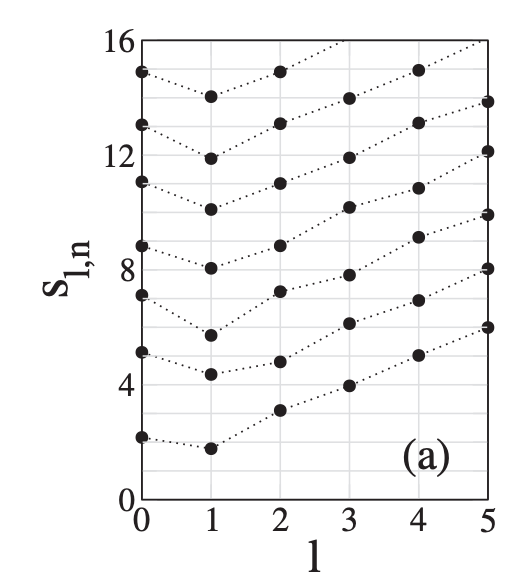
\includegraphics[width=0.5\textwidth]{chap13fSv.png}
    \bicaption{幺正极限下$\uparrow\downarrow\uparrow$三体体系$s_{l,n}$数值结果。摘自\cite{Fleix2006prlunitary3b} }{Numerical $s_{l,n}$ of $\uparrow\downarrow\uparrow$ three fermion system under unitary limit. Reprinted from \cite{Fleix2006prlunitary3b}}
    \label{Sv}
\end{figure}
将解到的$s_{l,n}$带入:
\begin{equation}
\left[-\frac{\hbar^{2}}{2 m}\left(\frac{d^{2}}{d R^{2}}+\frac{1}{R} \frac{d}{d R}\right)+U(R)\right] F(R)=\left(E-E_{\mathrm{c} . \mathrm{m} .}\right) F(R)
\end{equation}
其中$U(R)=\hbar^{2} s^{2} /\left(2 m R^{2}\right)+m \omega^{2} R^{2} / 2$。即可求得三体本征解。

基于上述框架,当s波相互作用处于幺正极限$a\to+\infty$时候,我们可以得到解析解,本征波函数为:
\begin{equation}
 F(R)=R^{s} e^{-R^{2} / 2 a_{\mathrm{ho}}^{2}} L_{q}^{(s)}\left(R^{2} / a_{\mathrm{ho}}^{2}\right)
\end{equation}
其中$a_{ho}=\sqrt{\hbar/m\omega}$,$s$为其中一个$s_{l,n}$,$L^{(\cdot)}_q$为q阶广义拉盖尔多项式,$q$为任意非负整数。能谱为:
\begin{equation}
E=E_{\mathrm{c} . \mathrm{m} .}+\left(s_{l, n}+1+2 q\right) \hbar \omega
\end{equation}

对于非幺正极限的相互作用情况,只能完全借助数值方法。Duan\cite{LmDuan2007levelcrossing}用格林函数的方法数值求解了整个相互作用区间。与上述框架稍有不同,哈密顿量为:
\begin{equation}
\begin{aligned}
&{\left[-\frac{\hbar^{2}}{m_{0}}\left(\nabla_{\mathbf{x}}^{2}+\nabla_{\mathbf{y}}^{2}\right)+\frac{1}{4} m_{0} \omega^{2}\left(\mathbf{x}^{2}+\mathbf{y}^{2}\right)-E\right] \Psi(\mathbf{x}, \mathbf{y})} \\
&\quad=-\sum V\left(\mathbf{r}_{\pm}\right) \Psi(\mathbf{x}, \mathbf{y})
\end{aligned}
\end{equation}
其中$\Vector{y}$为两个$\uparrow$费米子间相对位置。$\frac{\sqrt{\Vector{x}}}{2}$为$\downarrow$费米子相对两$\uparrow$费米子质心的相对位置。波函数在氢原子本征基矢下下展开,求解格林函数并利用边界条件,其中$\Vector{r}_{\pm}=\sqrt{3} \Vector{x} / 2 \pm \Vector{y} / 2$。
\begin{equation}
\begin{aligned}
&\Psi(\Vector{x}, \Vector{y})= \int d \Vector{x}^{\prime} d \Vector{y}^{\prime} G_{E}^{(2)}\left(\Vector{x}, \Vector{y} ; \Vector{x}^{\prime}, \Vector{y}^{\prime}\right)\times \sum_{\pm} \frac{\mp \hbar^{2} f\left(\Vector{r}^{\prime}{ }_{\perp, \pm}\right)}{m_{0}} \delta\left(\Vector{r}^{\prime}{ }_{\pm}\right)\\
&G_{E}^{(2)}\left(\mathbf{x}, \Vector{y} ; \mathbf{x}^{\prime}, \Vector{y}^{\prime}\right)=\sum_{\lambda_{1} \lambda_{2}} \frac{\psi_{\lambda_{1}}(\Vector{x}) \psi_{\lambda_{2}}(\Vector{y}) \psi_{\lambda_{1}}^{*}\left(\Vector{x}^{\prime}\right) \psi_{\lambda_{2}}^{*}\left(\Vector{y}^{\prime}\right)}{E_{\lambda_{1}}+E_{\lambda_{2}}-E}\\
\end{aligned}
\end{equation}
其中$\psi_\lambda(\Vector{r}) = R_{nl}(r)Y_l^m(\theta,\phi)$,$\lambda = (n,l,m),n=0,1,2...,l=0,1,2...$,$\Vector{r}_{\perp, \pm}=\Vector{x} / 2 \mp \sqrt{3} \Vector{y} / 2$边界条件为:
\begin{equation}
\Psi(\Vector{x}, \Vector{y}) \simeq \mp \frac{f\left(\Vector{r}_{\perp, \pm}\right)}{4 \pi \Vector{r}_{\pm}}\left(1-\frac{\mathbf{r}_{\pm}}{a}\right) \text { for } \Vector{r}_{\pm} \rightarrow 0
\end{equation}
进一步将$f\left(\mathbf{r}_{\perp}\right)$展开:
\begin{equation}
f\left(\mathbf{r}_{\perp}\right)=\Sigma_{\lambda} f_{\lambda} \psi_{\lambda}\left(\mathbf{r}_{\perp}\right)
\end{equation}
得到$f_\lambda$满足的矩阵方程:
\begin{equation}
\sum_{\lambda^{\prime}} A_{\lambda^{\prime}} f_{\lambda^{\prime}}=\left[\frac{d}{a}-2 \frac{\Gamma\left(\frac{3 / 2+E_{\lambda} / \hbar \omega-E / \hbar \omega}{2}\right)}{\Gamma\left(\frac{1 / 2+E_{\lambda} / \hbar \omega-E / \hbar \omega}{2}\right)}\right] f_{\lambda},
\end{equation}
其中:
\begin{equation}
A_{\lambda \lambda^{\prime}}=\int \frac{d \mathbf{r}_{\perp}}{4 \pi d^{3} \hbar \omega} G_{E-E_{\lambda^{\prime}}}\left(\frac{\sqrt{3} \mathbf{r}_{\perp}}{2}, 0\right) \psi_{\lambda}^{*}\left(\mathbf{r}_{\perp}\right) \psi_{\lambda^{\prime}}\left(\frac{-\mathbf{r}_{\perp}}{2}\right)
\end{equation}
最终得到能谱如图~\ref{duancrossing}~所示,通过跟两体能量的比较作者进一步发现了能级交叉。
\begin{figure}[!htbp]
    \centering
    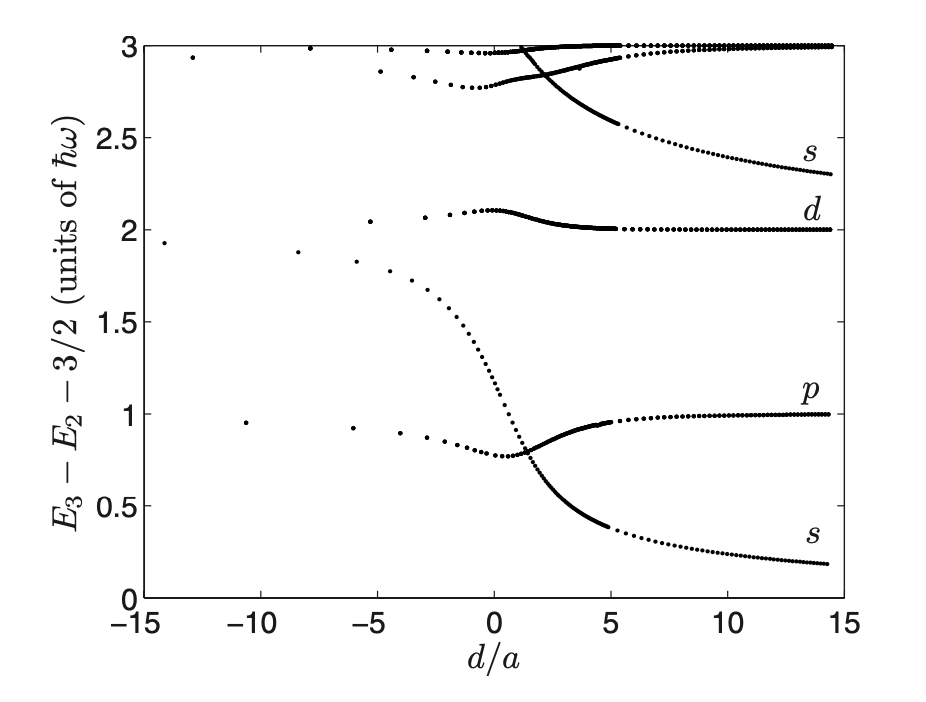
\includegraphics[width=0.7\textwidth]{chap1duan.png}
    \bicaption{三维下三费米子体系$\uparrow\downarrow\uparrow$能谱。摘自\cite{LmDuan2007levelcrossing}}{Spectrum
     of three fermions system($\uparrow\downarrow\uparrow$) in 3D. Reprinted from \cite{LmDuan2007levelcrossing}}
    \label{duancrossing}
\end{figure}

后续研究者\cite{Xiaji2009prl}则用两体本征波函数作为基矢展开求解了整个相互作用区间的严格解,其采用的展开波函数为:
\begin{equation}
\begin{split}
\psi_{3 b}^{\mathrm{rel}}(\mathbf{r}, \rho)&=\left(1-\mathcal{P}_{13}\right) \chi(\mathbf{r}, \rho)\\
\chi(\mathbf{r}, \rho)&=\sum a_{n} \psi_{2 b}^{\mathrm{rel}}\left(r ; v_{l, n}\right) R_{n l}(\rho) Y_{l}^{m}(\hat{\rho})\\
\end{split}
\end{equation}
其中$\psi_{2 b}^{\mathrm{rel}}$代表费米子1,2相对运动的波函数,对应能量为$E_{2b}=(2v_{l,n}+3/2)\hbar\omega$,而$R_{nl}(\rho Y^m_l(\hat{\rho}))$,其中$l,m$是系统的好量子数,代表了相对角动量与其沿z方向的分量。其物理图像非常清晰,将其中一个$\uparrow$费米子与$\downarrow$费米子结合在一起成为二聚体,第三个费米子相对于这个二聚体的运动由$a_n$所描述。最终求解方程:
\begin{equation}
\begin{split}
&\frac{2 \Gamma\left(-v_{l, n}\right)}{\Gamma\left(-v_{l, n}-1 / 2\right)} a_{n}+\frac{(-1)^{l}}{\sqrt{\pi}} \sum_{n^{\prime}} C_{n n^{\prime}} a_{n^{\prime}}=\left(\frac{d}{a}\right) a_{n}\\
&C_{n n^{\prime}} \equiv \int_{0}^{\infty} \rho^{2} d \rho R_{n l}(\rho) R_{n^{\prime} l}\left(\frac{\rho}{2}\right) \psi_{2 b}^{\mathrm{rel}}\left(\frac{\sqrt{3} \rho}{2} ; v_{l, n^{\prime}}\right)\\
\end{split}
\end{equation}
其能谱如图~\ref{xiaji3d}~所示。
\begin{figure}[!htbp]
    \centering
    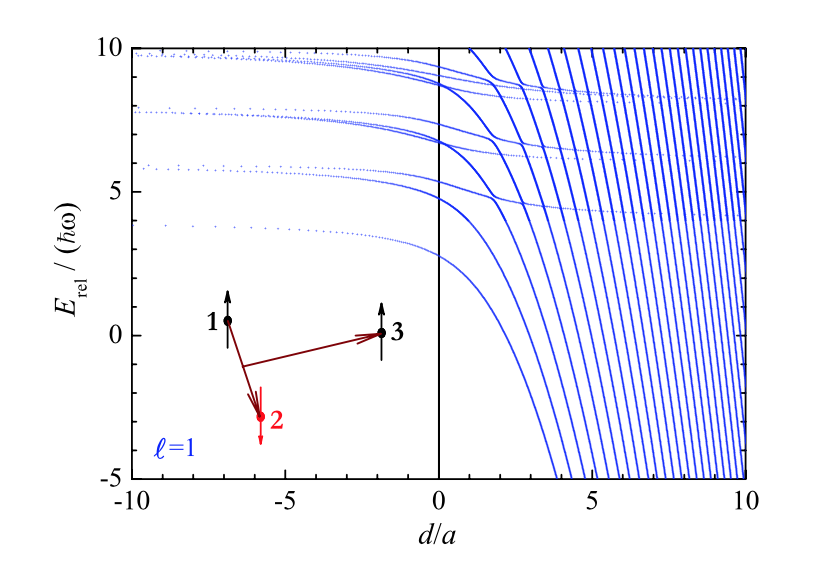
\includegraphics[width=0.7\textwidth]{chap1xiaji.png}
    \bicaption{二维下三费米子体系$\uparrow \downarrow \uparrow$的能谱。摘自\cite{Xiaji2009prl}}{Spectrum of three fermion system($\uparrow\downarrow\uparrow$ in 3D. Reprinted from \cite{Xiaji2009prl}}
    \label{xiaji3d}
\end{figure}
与此同时,研究者Xiaji\cite{Xiaji20103b}还研究了二维体系下,三体精确解,采用类似的办法,
\begin{equation}
\begin{split}
\psi_{3 f}^{r e l}&=\left(1-\mathcal{P}_{13}\right) \chi(\mathbf{r}, \vec{\rho})\\
\chi(\mathbf{r}, \vec{\rho})&=\sum_{n} a_{n}^{f} \psi_{2 p}^{r e l}\left(\mathbf{r} ; \nu_{m, n}\right) R_{n m}(\rho) \frac{e^{i m \varphi}}{\sqrt{2 \pi}}\\
\end{split}
\end{equation}
得到整个相互作用的能谱。同时Blume研究了从三维到二维一维的渡越\cite{blume2012},通过各项异性的谐振子束缚体系的求解来研究维度的渡越。

而在严格一维体系里面,三费米子的严格求解则由\cite{Rittenhouse2010green,d2014three,loft2015variational,andersen2016interpolatory,bellotti2017comparing}给出。
采用的波函数为:
\begin{equation}
\begin{split}
\psi_{3 F}(x, y)&=\left(1-\boldsymbol{P}_{13}\right) \Omega(x, y)\\
\Omega(x, y)&=\sum_{n=0}^{\infty} a_{n} \psi_{n}^{2b}(x) R_{n}(y)\\
\psi_{n}^{2b}(x)&=\Gamma\left(-v_{n}\right) \mathrm{e}^{-\frac{x^{2}}{2}} U\left(-v_{n}, \frac{1}{2}, x^{2}\right)\\
\end{split}
\end{equation}
其中$\psi_{n}^{2b}(x)$为两体相互作用在谐振势中的解,$R_{n}(y)$为谐振子的本征解。类似地,带入到Bethe–Peierls边界条件中得到耦合方程:
\begin{equation}
\begin{aligned}
&2 g \sum_{n} a_{n}\left[\sqrt{\pi} \frac{\Gamma\left(-v_{n}\right)}{\Gamma\left(-v_{n}+1 / 2\right)} R_{n}(y)-\psi_{n}\left(\frac{\sqrt{3}}{2} y\right) R_{n}\left(-\frac{y}{2}\right)\right] \\
&=-4 \sqrt{\pi} \sum_{n} a_{n} R_{n}(y)
\end{aligned}
\end{equation}
相应地能谱如图~\ref{1d3b}~所示。
\begin{figure}[!htbp]
    \centering
    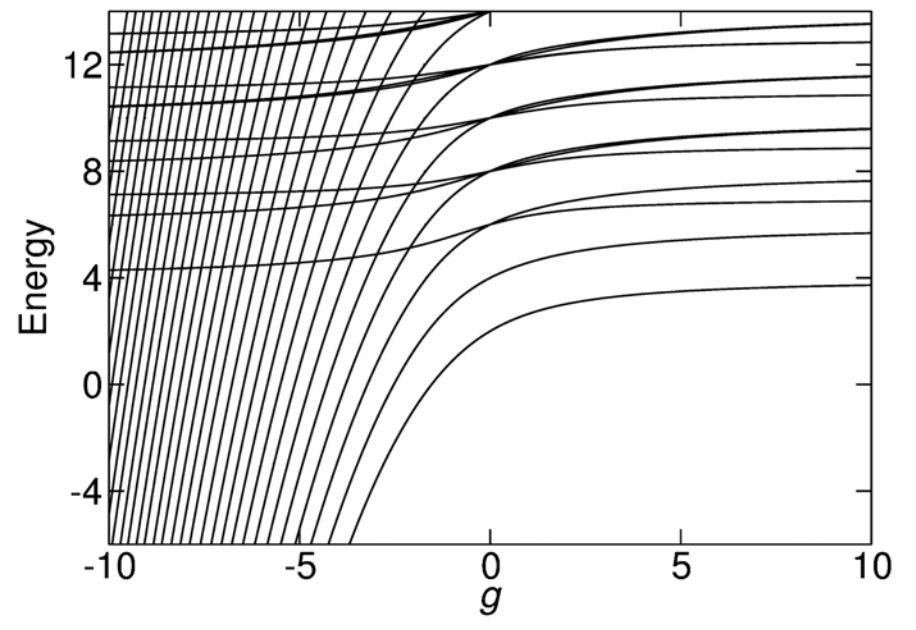
\includegraphics[width=0.7\textwidth]{chap11d3b.png}
    \bicaption{一维下三费米子体系$\uparrow \downarrow \uparrow$的能谱。摘自\cite{d2014three} }{Spectrum of three fermion system($\uparrow\downarrow\uparrow$ in 1D. Reprinted from \cite{d2014three}}
    \label{1d3b}
\end{figure}

继续增加粒子的数目到四体甚至五体,有一些数值结果\cite{Blume2010,blume2012few},不过如何有效地求解这类体系依然是一个开放问题。多粒子体系中唯一的有个例外就是在严格一维时候,我们知道可以用贝特假设求解,通常情况下贝特假设结果的物理意义不容易提取。但是在某些极限下却有清楚的物理图像,这其中一个典型例子就是Tonks极限及其附近的自旋链模型\cite{Guan2009exact,ma2009mathematical,Lewenstein2013spinchain,volosniev2014strongly,Busch013spinchain,CuiHo2014,Santos2014spinchain,Puhan2015spinchain,Yang2016effective}。该模型说的是首先对于无限大相互作用的自旋1/2费米子体系,受到Girardeau 处理玻色子的启发,Guan严格求解了自旋费米子体系的严格解\cite{Guan2009exact}。其中基态简并是一重要特征。定义N个费米子在一维顺序自旋排布$\xi_{1}, \xi_{2}, \ldots, \xi_{N}$态为:
\begin{equation}
\left|\left\{\xi_{1}, \xi_{2}, \ldots, \xi_{N}\right\}\right\rangle \equiv|\vec{\xi}\rangle
\end{equation}
其坐标表示为:
\begin{equation}
\begin{aligned}
&\langle x_{1}, \ldots, x_{N} ; \mu_{1}, \ldots, \mu_{N} \mid \vec{\xi}\rangle \\
&\quad=\sum_{P} \theta\left(x_{P_{1}}, x_{P 2}, \ldots, x_{P_{N}}\right) \prod_{i} \delta_{\xi_{i}, \mu_{P_{i}}}
\end{aligned}
\end{equation}
其中$P$为$(1,2..,N)$的一个置换。并且:
\begin{equation}
\begin{aligned}
\theta\left(x_{P_{1}}, x_{P 2}, \ldots, x_{P_{N}}\right) &=1 & & \text { 如果 } x_{P_{1}}<x_{P 2}<\cdots<x_{P_{N}} \\
&=0 & & \text { 其它 }
\end{aligned}
\end{equation}
由于体系相互作用仅存在于不同自旋费米子之间,因此总的自旋$\Vector{S}_{tot},S_{tot,z}$守恒。N个费米子在共振点出发生费米化,相互作用转变为边界条件:
\begin{equation}
\left.\Psi\left(x_{1}, \sigma_{1} ; \ldots ; x_{N}, \sigma_{N}\right)\right|_{x_{i}=x_{j}, \sigma_{i}=-\sigma_{j}}=0
\end{equation}
如果其中$M$个$\uparrow$,$N-M$个$\downarrow$,本征波函数具有$C_N^M$重简并:
\begin{equation}
\begin{split}
&\Psi_{F}^{\xi}=\phi_{F}\left(x_{1}, x_{2}, \ldots, x_{N}\right)\langle x_{1}, \ldots, x_{N} ; \mu_{1}, \ldots, \mu_{N} \mid \vec{\xi}\rangle\\
&\phi_{F}\left(x_{1}, x_{2}, \ldots, x_{N}\right) =\frac{1}{\sqrt{N !}} D\left(x_{1}, x_{2}, \ldots, x_{N}\right) \\
&\quad\quad =\prod_{i<j}\left(x_{i}-x_{j}\right) F\left(x_{1}, x_{2}, \ldots, x_{N}\right)\\
\end{split}
\end{equation}
其中$\phi_F$由N个不同谐振子能级波构成。一旦相互作用不在共振处,这些简并的能级就会打开简并,其打开简并的方式恰好可以被自旋链模型所描述。
\begin{equation}
H_{\mathrm{eff}}=\sum_{l} \frac{J_{l}}{g}\left(\mathbf{s}_{l} \cdot \mathbf{s}_{l+1}-\frac{1}{4}\right)
\end{equation}
其中自旋之间的耦合常数满足:
\begin{equation}
J_{l}=\left.2 N !\left(\frac{1}{m}\right)^{2} \int d \mathbf{x}\left|\frac{\partial \phi_{F}}{\partial x_{i j}}\right|_{x_{i j}=0}\right|^{2} \theta\left(\cdots<x_{i}=x_{j}<\cdots\right)
\end{equation}
具体的计算参见\cite{Guan2009exact,Santos2014spinchain,Yang2016effective}
\begin{figure}[!htbp]
    \centering
    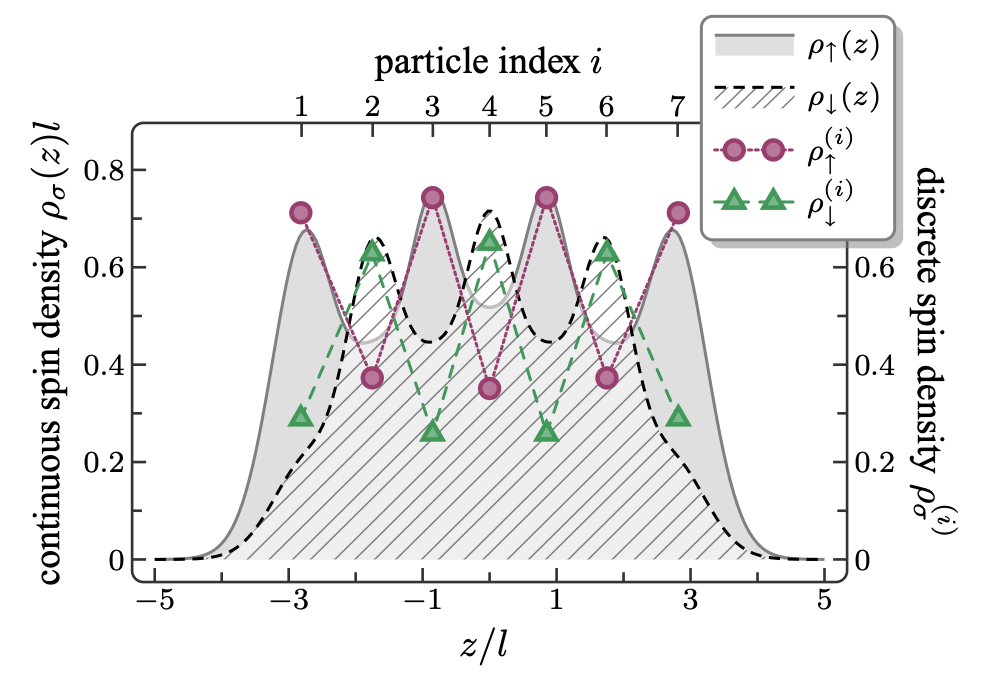
\includegraphics[width=0.7\textwidth]{chap1spinchainth.png}
    \bicaption{少体自旋1/2费米子体系无限大排斥附近的自旋链有效模型。摘自\cite{Santos2014spinchain} }{Spin-chain representation of an infinitely repulsive system of a few fermions. Reprinted from \cite{Santos2014spinchain}}
    \label{spinchainth}
\end{figure}

有了上面介绍的量子少体研究进展,将有几个可扩展的方向,比如改变相互作用,dipole、库伦、以及自旋交换相互作用,这其中自旋交换相互作用将是下一章节要重点介绍的。

\section{自旋交换相互作用}\label{sec:spin-exchange}
在超冷原子实验平台中,原子整体作为基本粒子,但是具有内禀自由度。分为内部电子轨道自由度和核自旋自由度。在冷原子实验平台发展初期,冷却囚禁的原子主要集中在碱金属一族,最外层只有一个电子。后续随着实验技术的进步,碱土金属一族的原子进入到大家的视野{\color{red} AE原子体系制备 }。这类冷原子最外层有两个电子,基态${}^1S_0$与激发态${}^3P_0$都具有较长的寿命(选择定则),称为轨道自由度。由于不同内部电子结构的原子间相互作用不同,因此不同轨道天然地带来了不同的原子间相互作用。进一步,由于体系温度极低,轨道电子的总角动量$J$为零,碱土金属元素的核自旋自由度可以发挥重大的作用。这就为碱土金属原子作为量子模拟的平台带来丰富的可能性。

最早在碱土金属中做量子模拟的可以追溯到2010年理论想法,基于当时对于费米型碱土金属原子的冷却与调控,A. V. Gorshkov\cite{gorshkov2010two}提出了利用这一平台来模拟SU(N)相关的物理。具体地,从两体散射来讲,原子间的相互作用仅与价电子排布有关而与核自旋无关。由于费米子的全同性原理,两体散射中轨道自由的与核自旋自由度整体满足交换反对称特性,因此两体散射通道分为

光晶格中费米型碱土金属原子服从的哈密顿量为:
\begin{equation}
\begin{aligned}
\hat{H}=& \sum_{\alpha m} \int \mathrm{d}^{3} \mathbf{r} \hat{\Psi}_{\alpha m}^{\dagger}(\mathbf{r})\left(-\frac{\hbar^{2}}{2 M} \nabla^{2}+V_{\alpha,opt}(\mathbf{r})\right) \hat{\Psi}_{\alpha m}(\mathbf{r}) \\
&+\hbar \omega_{0} \int \mathrm{d}^{3} \mathbf{r}\left(\hat{\rho}_{e}(\mathbf{r})-\hat{\rho}_{g}(\mathbf{r})\right)+ \sum_{\alpha, m<m^{\prime}} g_{\alpha \alpha} \int \mathrm{d}^{3} \mathbf{r} \hat{\rho}_{\alpha m}(\mathbf{r}) \hat{\rho}_{\alpha m^{\prime}}(\mathbf{r})  \\
&+ g_{e g^+} \int \mathrm{d}^{3} \mathbf{r} \hat{\rho}_{eg^+}(\mathbf{r}) \hat{\rho}_{eg^+}(\mathbf{r})+g_{e g^-} \int \mathrm{d}^{3} \mathbf{r} \hat{\rho}_{eg^-}(\mathbf{r}) \hat{\rho}_{eg^-}(\mathbf{r})\\
\end{aligned}
\end{equation}
其中$\alpha=g({^1S_0})$或者$e({}^3P_0)$代表不同电子内态的原子。$m=-I,...,I$对应核自旋分量。$eg^+$与$eg^-$对应散射通道:
\begin{equation}
|eg^{\pm}\rangle = \frac{|ge\rangle\pm|eg\rangle}{\sqrt{2}}\otimes\frac{|\uparrow\downarrow\rangle\mp|\downarrow\uparrow \rangle}{\sqrt{2}}
\end{equation}

由于因此表征原子间相互作用参数仅需要四个通道的相互作用常数$g_{gg},g_{ee},g_{eg^+},g_{eg^-}$。如图~\ref{eg}~
\begin{figure}[!htbp]
    \centering
    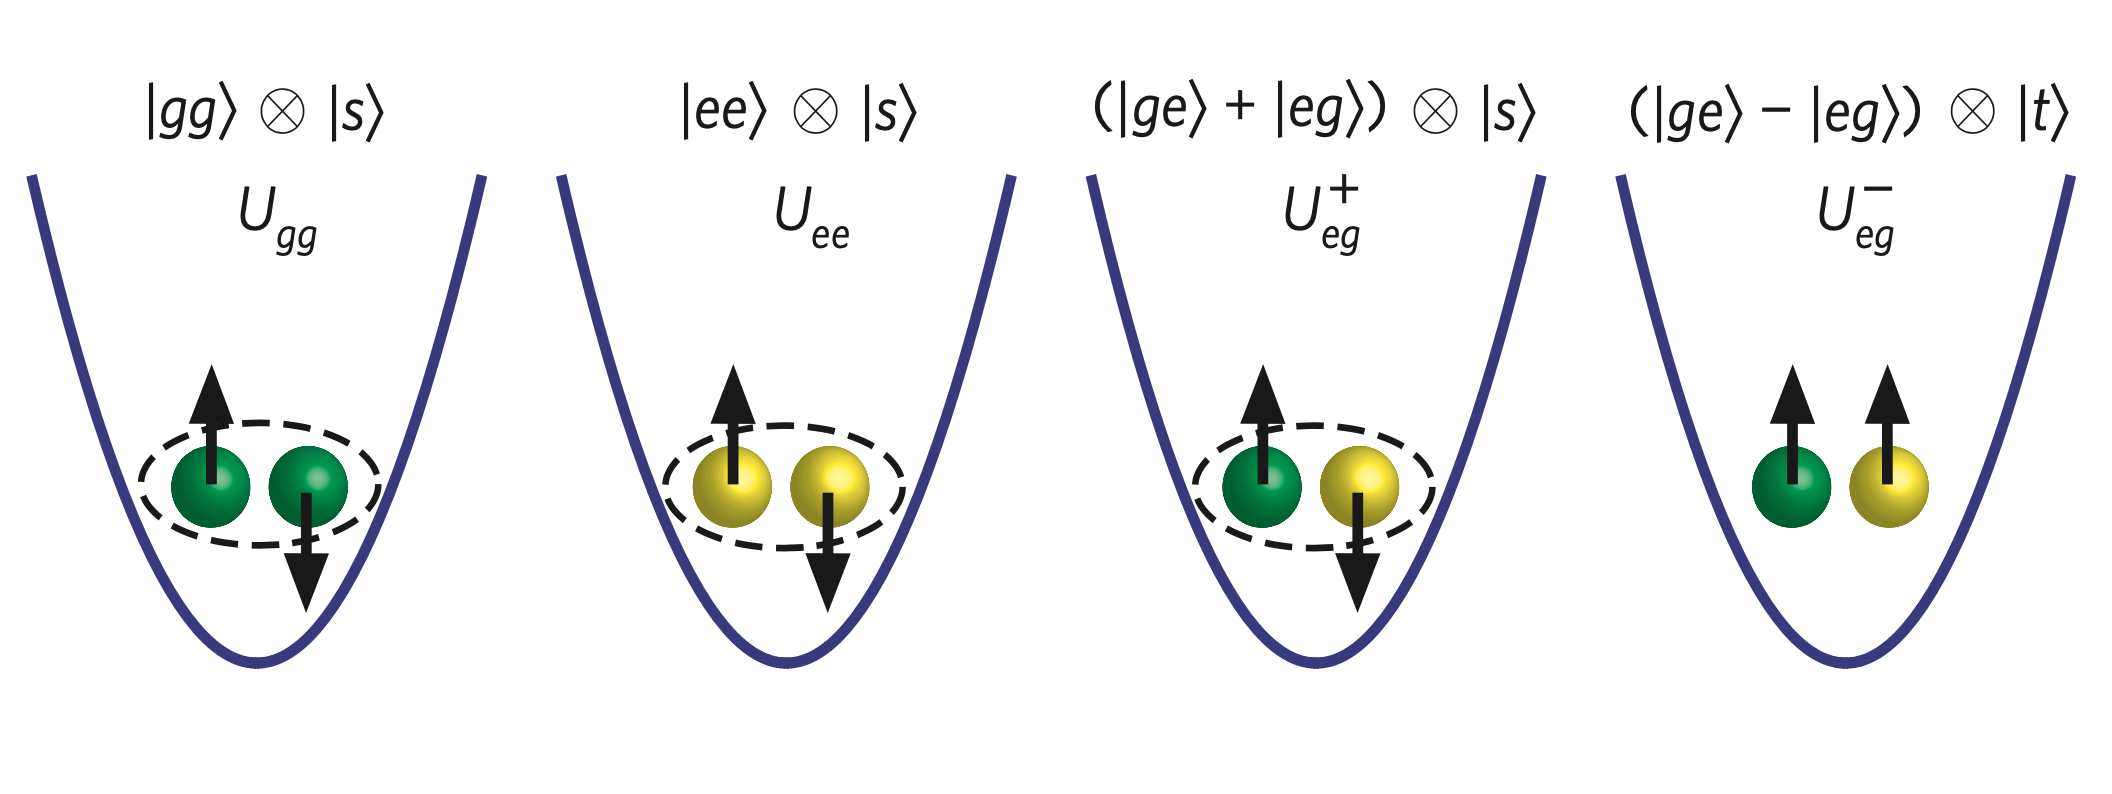
\includegraphics[width=0.7\textwidth]{eg.png}
    \bicaption{摘自SU(N)}{Reprinted from SU(N)}
    \label{eg}
\end{figure}
如果将$\hat{\rho}_{eg^\pm}$展开,我们得到不同轨道原子间的相互作用$\hat{V}_{eg}$分成了自旋交换与自旋守恒的两项:
\begin{equation}
\begin{aligned}
\hat{V}_{eg^+} &= g_{e g^+} \int \mathrm{d}^{3} \mathbf{r} \hat{\rho}_{eg^+}(\mathbf{r}) \hat{\rho}_{eg^+}(\mathbf{r})+g_{e g^-} \int \mathrm{d}^{3} \mathbf{r} \hat{\rho}_{eg^-}(\mathbf{r}) \hat{\rho}_{eg^-}(\mathbf{r})\\
\quad &= \frac{g_{e g}^{+}+g_{e g}^{-}}{2} \int \mathrm{d}^{3} \mathbf{r} \rho_{e}(\mathbf{r}) \rho_{g}(\mathbf{r}) \\ 
&\quad \quad + \frac{g_{e g}^{+}-g_{e g}^{-}}{2} \sum_{m m^{\prime}} \int \mathrm{d}^{3} \mathbf{r} \Psi_{g m}^{\dagger}(\mathbf{r}) \Psi_{e m^{\prime}}^{\dagger}(\mathbf{r}) \Psi_{g m^{\prime}}(\mathbf{r}) \Psi_{e m}(\mathbf{r})
\end{aligned}
\end{equation}
最后,将整个二次量子化哈密顿量在光晶格紧束缚近似下写为:
\begin{equation}
\begin{aligned}
\hat{H}=&-\sum_{\langle j, i\rangle \alpha, m} J_{\alpha}\left(c_{i \alpha m}^{\dagger} c_{j \alpha m}+\text { h.c. }\right)+\sum_{j, \alpha} \frac{U_{\alpha \alpha}}{2} n_{j \alpha}\left(n_{j \alpha}-1\right) \\
&+V \sum_{j} n_{j e} n_{j g}+V_{e x} \sum_{j, m, m^{\prime}} c_{j g m}^{\dagger} c_{j e m^{\prime}}^{\dagger} c_{j g m^{\prime}} c_{j e m}
\end{aligned}
\end{equation}
其中$\hat{n}_{j\alpha}=\sum_m \hat{n}_{j\alpha m}$,$V=\left(U_{e g}^{+}+U_{e g}^{-}\right) / 2$与$V_{ex}=\left(U_{e g}^{+}-U_{e g}^{-}\right) / 2$分别描述不同轨道原子间的自旋不变与自旋交换相互作用,其中:
\begin{equation}
U_{eg^\pm} = g_{eg^\pm} \int \mathrm{d}^{3} \mathbf{r} w_e^2(\mathbf{r})w_g^2(\mathbf{r})
\end{equation}
有了上述丰富的轨道间相互作用与核自旋SU(N)自由度,这一模型可以用来模拟众多凝聚态物理中强关联多体模型,比如近藤晶格模型、自旋链模型、自旋液体等。

紧接着于2014年,F. Scazza\cite{scazza2014observation}与合作者一起在${}^{173}$Yb体系中证实了上述自旋交换相互作用的存在。其思路如图~\ref{egexp}~所示:
\begin{figure}[!htbp]
    \centering
    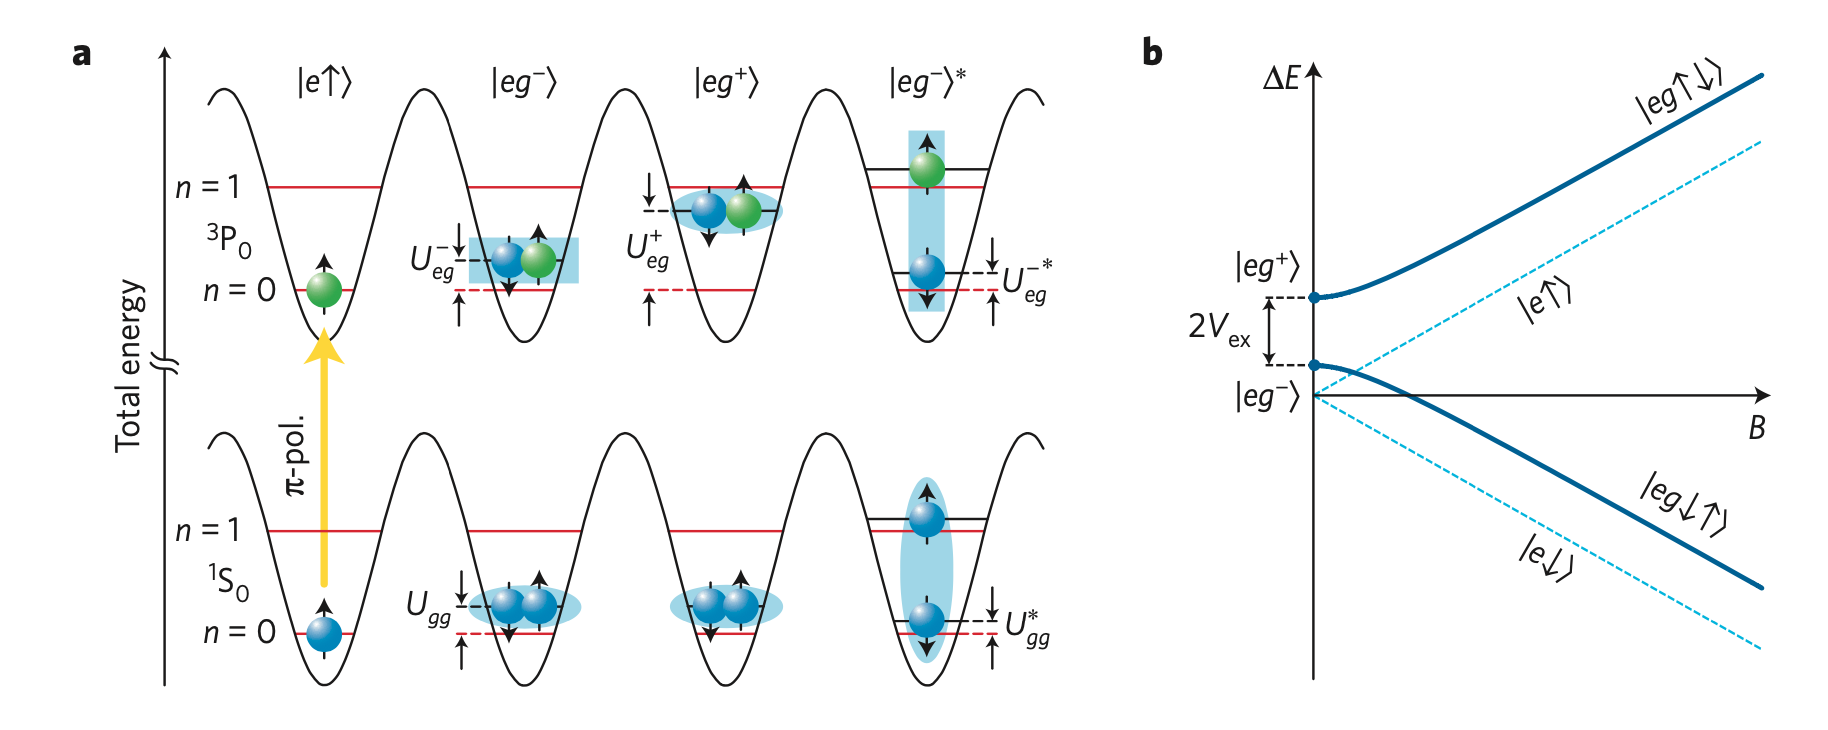
\includegraphics[width=0.7\textwidth]{egexp.png}
    \bicaption{图A代表单原子与双原子初态到末态的跃迁。图B代表末态的能谱。摘自\cite{scazza2014observation}}{Fig.(A) for transition from initail state to final state under laser field. Fig(B) for energy spectrum of final state. Reprinted from \cite{scazza2014observation}}
    \label{egexp}
\end{figure}
该实验选取不同电子排布($g({}^1S_0)$与$e({}^3P_0)$)的${}^{173}$Yb($I=5/2$)原子,束缚在较深(原子不能自由移动)的光晶格中,在每个格点里面,原子间的相互作用能为:
\begin{equation}
U_{X}=\frac{4 \pi \hbar^{2}}{m} a_{X} \int \mathrm{d}^{3} r w_{a}^{2}(\mathbf{r}) w_{b}^{2}(\mathbf{r})
\end{equation}
其中$X =gg, ee, eg^+, eg^−$代表不同状态的原子对。装载不同核自旋的$g$轨道原子到光晶格中,平均填充在$\bar{n}=1$与$\bar{n}=2$之间,这样导致部分格点内有一个原子,部分格点内有两个原子。对于有两个原子的格点,用激光将一个原子从g态激发到e态,末态有两个本征态$|eg^\pm\rangle$,本征能量为$U_{eg^\pm}$。如果在体系中加入沿$z$方向的磁场,导致$|eg^\pm\rangle$两态之间有非零的跃迁矩阵元,最终的哈密顿量为:
\begin{equation}
H_{e g}=\left(\begin{array}{cc}
U_{e g}^{+} & \Delta_{B} \\
\Delta_{B} & U_{e g}^{-}
\end{array}\right)
\end{equation}
其中$\Delta_{B}=\delta g m_{\mathrm{F}} \mu_{\mathrm{B}} B$,$\delta g$为核自旋朗德因子的差值,跃迁末态的本征能量为:
\begin{equation}
E_{1,2}=V \pm \sqrt{V_{\mathrm{ex}}^{2}+\Delta_{B}^{2}}
\end{equation}
本征波函数为$|eg^\pm\rangle$两态的线性叠加。

通过观测不同磁场下的共振谱,得到不同磁场下末态的能量。进一步地,通过测量初态自旋分布到末态自旋分布演化\cite{scazza2014observation,cappellini2014direct},直接观测到了自旋交换相互作用。如图~\ref{egd}~
\begin{figure}[!htbp]
    \centering
    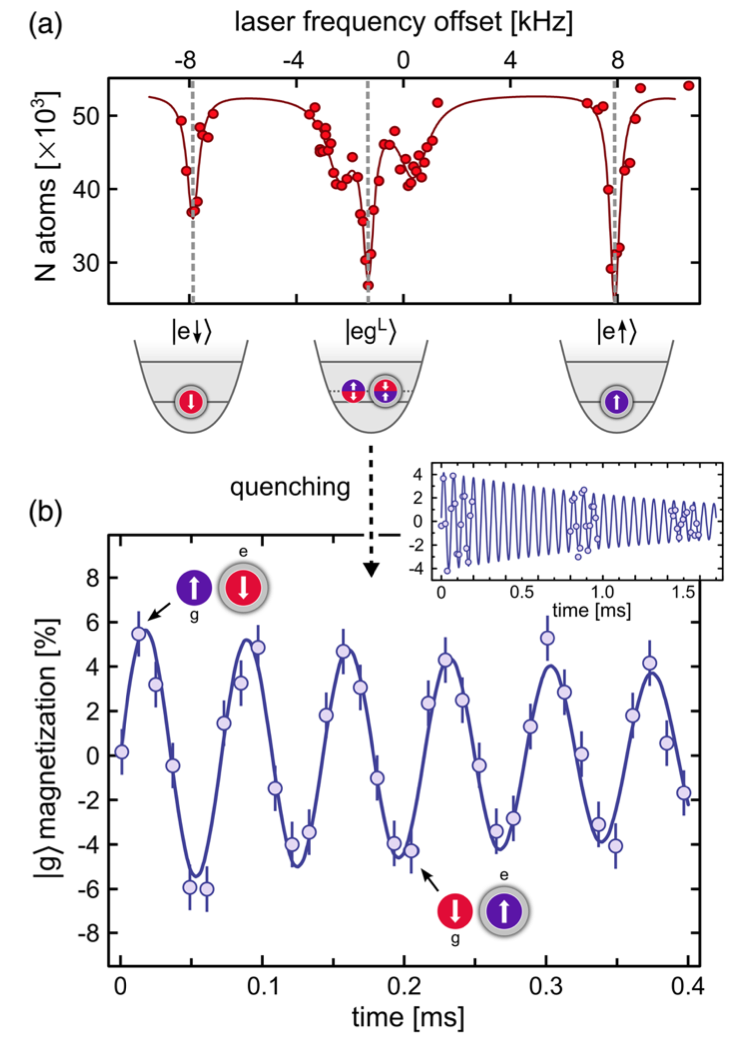
\includegraphics[width=0.6\textwidth]{chap1spexd.png}
    \bicaption{图a代表实验测到的吸收谱,不同的峰代表了不同的末态。图b代表观测到自旋交换体系的的自旋动力学。摘自\cite{cappellini2014direct}}{Fig(A) for spectrum of clock transition. Fig(B) for time resolved spin transition. dynamics. Reprinted from \cite{cappellini2014direct}}
    \label{egd}
\end{figure}
拟合实验中不同磁场下测到的共振峰的位置,最终测到${}^{173}$Yb原子间裸的散射长度为\cite{scazza2014observation,cappellini2014direct}:
\begin{equation}
\begin{split}
a_{e g}^{+}&=(3300 \pm 300) a_{0}\\
a_{e g}^{-}& = 219.5 a_0\\
\end{split}
\end{equation}
可以看到为铁磁耦合。与此同时,来自研究者也分别在中观测到了Sr原子体系的铁磁自旋交换相互作用\cite{zhang2014spectroscopic}。

但是上述观测到的裸的原子间相互作用为铁磁自旋耦合,模拟近藤物理需要反铁磁耦合。这时候理论研究者提出利用束缚诱导共振来调节。一系列系统的工作表明利用束缚诱导共振来调节反铁磁自旋交换的强度\cite{zhang2016kondo,cheng2017enhancing,zhang2018control,ji2018confinement,zhang2020tight,zhang2020controlling}。最终实验上成功观测到了的准一维体系束缚诱导增强的自旋动力学\cite{riegger2018localized}。
\begin{figure}[!htbp]
    \centering
    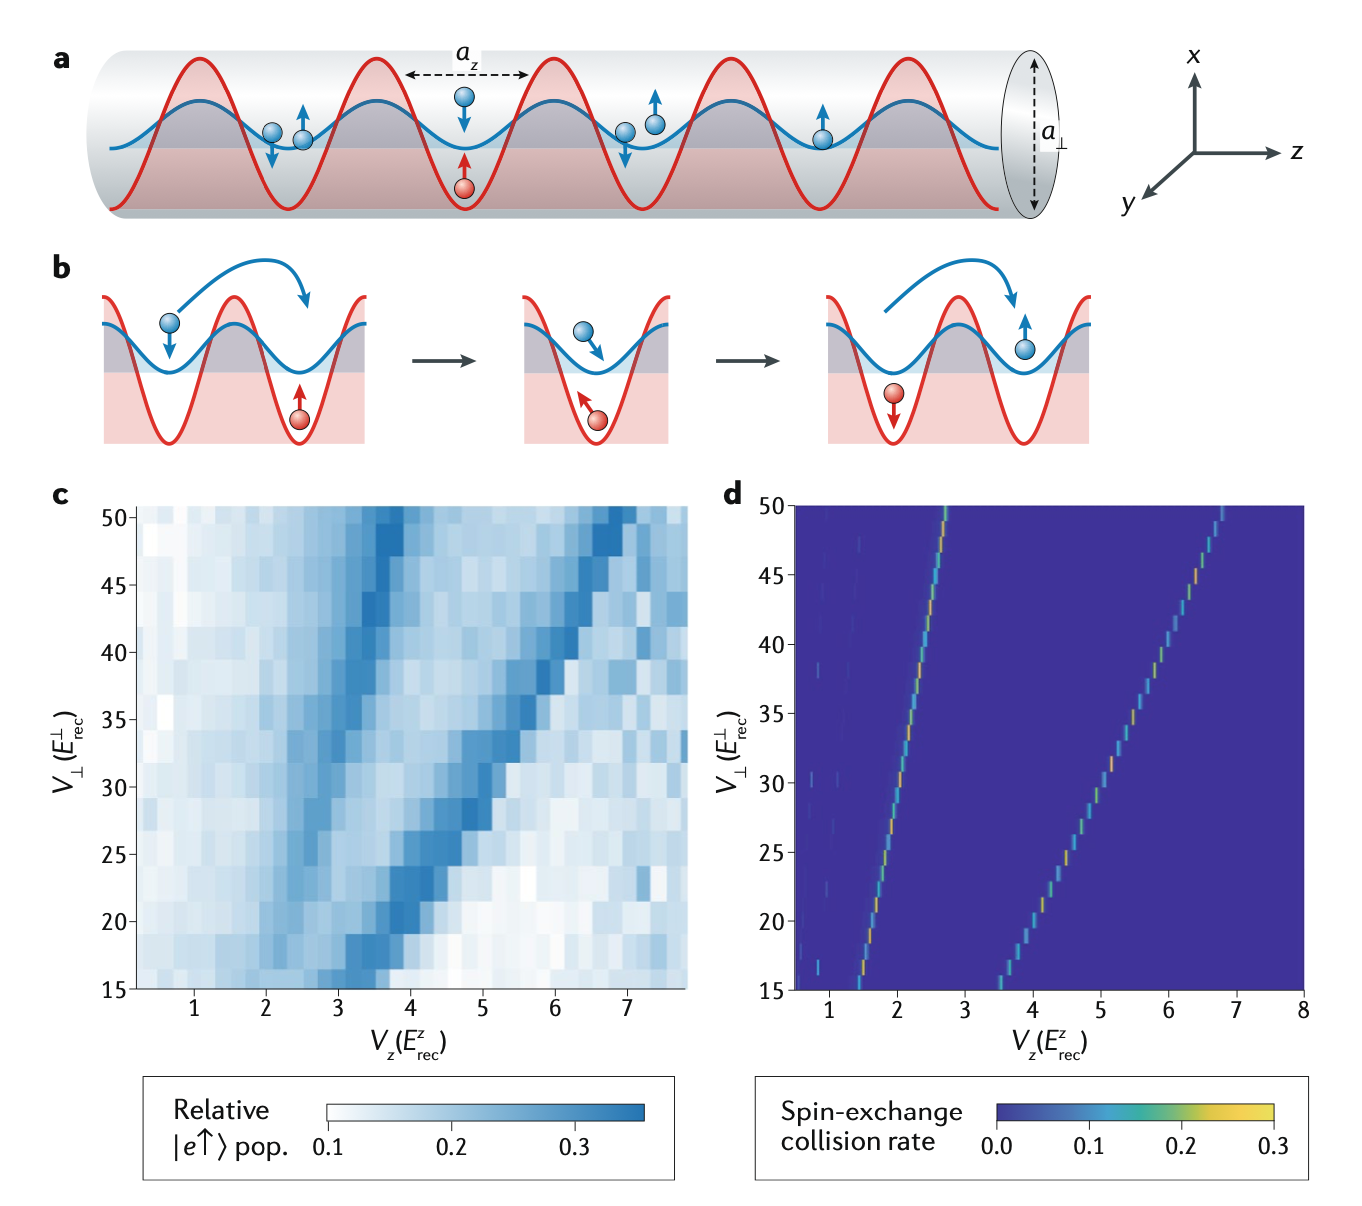
\includegraphics[width=0.7\textwidth]{chap1spexCIR.png}
    \bicaption{图a代表准一维体系z方向上自旋相关的晶格制造巡游费米子与局域费米子。图b代表自旋交换发生的过程。图c,d分别代表实验测量与理论预测的束缚诱导增强下的自旋交换动力学。摘自\cite{riegger2018localized,zhang2020controlling}}{Fig(a) for quasi 1D system, which consists of spin-dependent lattice to creat free hopping fermions and localized spin. Fig(b) for illustration of spin exchange process. Fig(c) for Experimental and theoretical spin exchange interaction enchanced by confinement induced resonance. Reprinted from \cite{riegger2018localized,zhang2020controlling}}
    \label{CIRspexexp}
\end{figure}


\section{极化子理论与实验}

极化子是一个杂质物理中比较古老的概念。早在固体物理中就有研究大极化子与小极化子\cite{landau1933bewegung,pekar1946autolocalization,frohlich1950xx,frohlich1954electrons,feynman1955slow,mahanmany},对应的是电子在晶格中运动,电子的单粒子性质被晶格声子激发所修饰,改变其有效质量、寿命等。严格说晶格里的极化子属于玻色极化子。如果将背景原子改为多体费米体系,就得到费米极化子。理论上,极化子是典型的费米液体。近年来,随着冷原子中Imblanced 费米混合气体的制备,极化子作为其中的极端体系,进入研究者的视野,结合冷原子体系特有的控制、操控、观测能力,极化子的研究迎来新的阶段,我们将围绕相关研究的实验与理论展开。
\begin{figure}[!htbp]
    \centering
    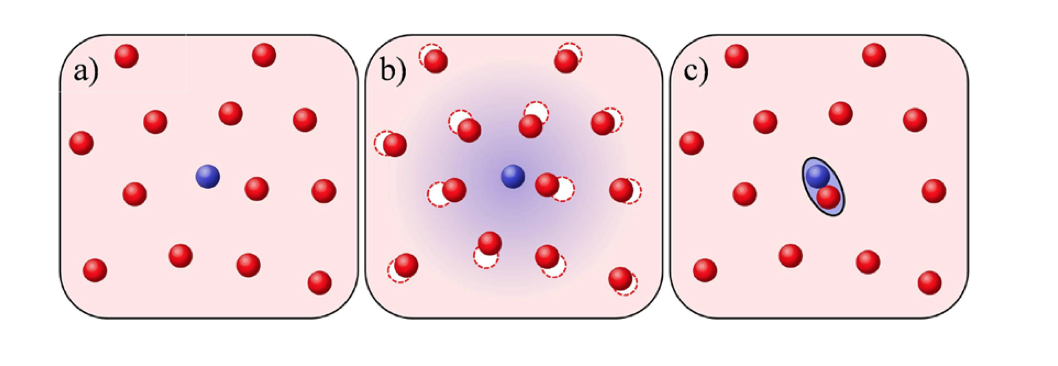
\includegraphics[width=0.7\textwidth]{chap1fp.png}
    \bicaption{费米极化子的示意图。相互作用从弱变强依次从极化子变到分子。摘自\cite{Schirotzekobservation}}{Illustration of fermi polaron. As interaction goes strong, impurity goes from polaron to molecule. Reprinted from \cite{Schirotzekobservation}p}
    \label{fp}
\end{figure}

\subsection{极化子实验}
超冷原子中极化子物理研究的启发来自于population-imblanced混合费米气体。其中少数原子成为杂质,多数原子构成背景。杂质原子的单粒子性质被背景费米海上的粒子-空穴激发所重整化,如图~\ref{fp}~所示。费米极化子最早的直接实验证据来自MIT研究组\cite{Schirotzekobservation}。实验上制备含有$10^6$个$|1\rangle{}^6$Li原子的体系。然后通过双光子过程将大约$2\%$的$|1\rangle$原子激发到$|3\rangle$。调节$|1\rangle$与$|2\rangle$之间的相互做作用,然后通过测量$3|\rangle$到$|2\rangle$的rf谱,通过谱峰的位置来给出极化子的能量,如图~\ref{fpE}~所示。
\begin{figure}[!htbp]
    \centering
    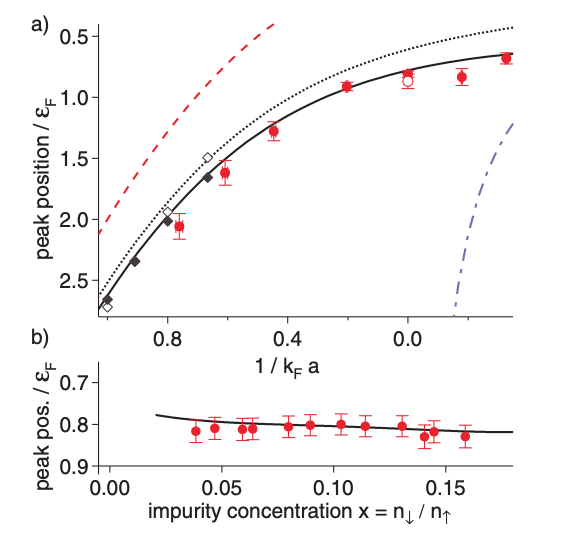
\includegraphics[width=0.7\textwidth]{chap1fpE.png}
    \bicaption{图a为实验测到的(散点)以及理论预测(黑色实线)的费米极化子能量随相互作用变化曲线。图b为rf谱峰的位置随杂质密度的变化。摘自\cite{Schirotzekobservation}}{Fig(a) for measured and predicted energy of fermi polaron upon interaction. Fig(b) for rf spectrum peak position upon impurity densuty. Reprinted from\cite{Schirotzekobservation}}
    \label{fpE}
\end{figure}

可以看到,即使在共振点处,理论计算的能量与实验测到的能量也符合很好。并且谱峰的位置受杂质密度变化影响较小,处于低密度区间。进一步分析rf谱的面积,提取出准粒子剩余,如图~\ref{fpZ}~所示。
\begin{figure}[!htbp]
    \centering
    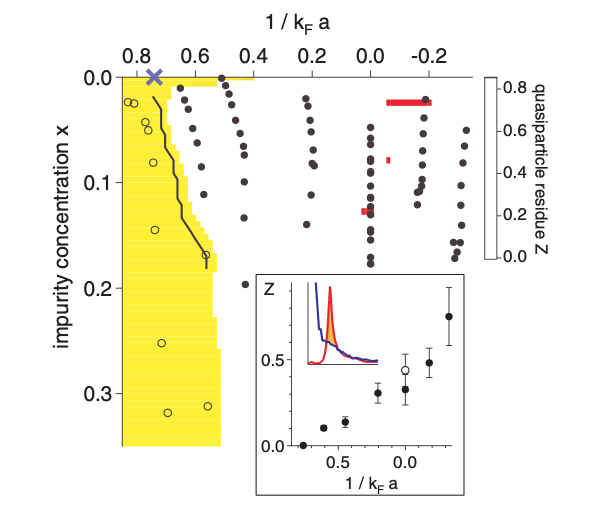
\includegraphics[width=0.6\textwidth]{chap1fpZ.png}
    \bicaption{准粒子剩余随着相互作用与密度的变化。摘自\cite{Schirotzekobservation}}{Quasiparticle residue as a function of interaction and impurity densuty. Reprinted from \cite{Schirotzekobservation}}
    \label{fpZ}
\end{figure}


进一步实验\cite{kohstall2012metastability}采用不同的体系,制备少量${}^{40}$K与大量${}^{6}$Li的混合气,通过rf pulse将与Li原子无相互作用的$|0\rangle\equiv\left|F=9 / 2, m_{\mathrm{F}}=-7 / 2\right\rangle$激发到与Li原子有Feshbach共振调节相互作用的$|1\rangle \equiv\left|F=9 / 2, m_{\mathrm{F}}=-5 / 2\right\rangle$。观测到在吸引极化子之上还有一支排斥极化子,这是一个激发态,杂质原子间的相互作用越过共振点,从低能有效散射角度来看杂质原子与背景之间互相排斥,其根源来自于少体体系里的upper branch。如图~\ref{upfp}~所示 :
\begin{figure}[!htbp]
    \centering
    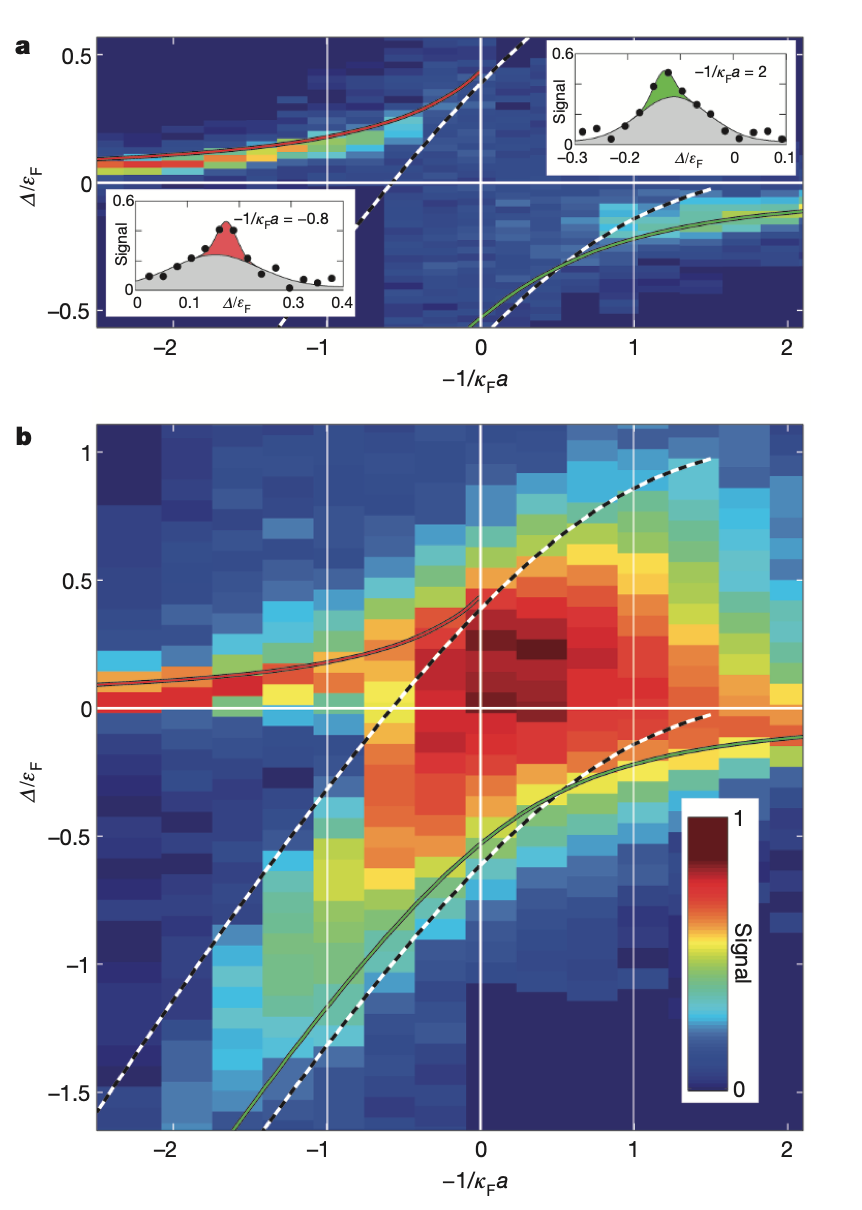
\includegraphics[width=0.6\textwidth]{chap1upfp.png}
    \bicaption{图a(弱)与b(强)为不同rf场强下测到的吸收谱。\cite{kohstall2012metastability}}{Fig(a) and Fig(b) for transition spectrum measured under weak and strong rf power. Reprinted from \cite{kohstall2012metastability}}
    \label{upfp}
\end{figure}
后续在纯${}^{6}$Li体系中也观测到了排斥极化子\cite{Scazzarepulsive}。

我们知道在低维体系中密度涨落会扮演更重要的角色。那对于二维体系的费米极化子会是如何呢?研究者在${}^{40}$K二维光晶格中实现了二维费米极化子,并观测到了attractive branch与repulsive branch。
降低维度观测到2D极化子low与up\cite{koschorreck2012attractive}。
\begin{figure}[!htbp]
    \centering
    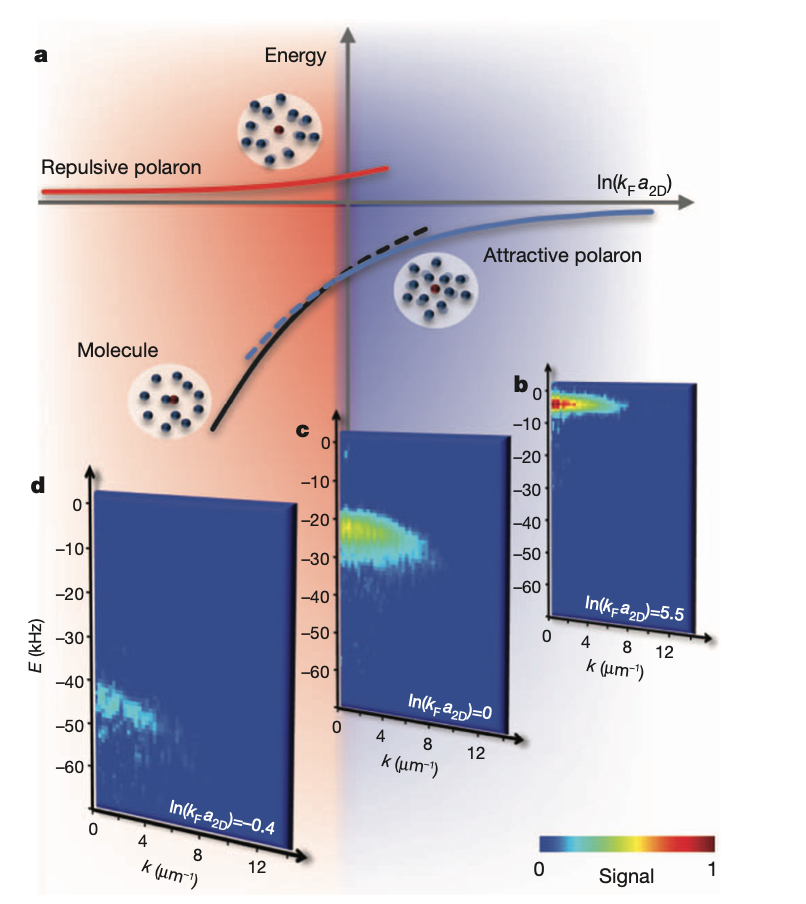
\includegraphics[width=0.7\textwidth]{chap12dfp.png}
    \bicaption{摘自SU(N) exp}{Reprinted from SU(N) exp}
    \label{2dfp}
\end{figure}

超快Ramesy spectroscopy
\begin{figure}[!htbp]
    \centering
    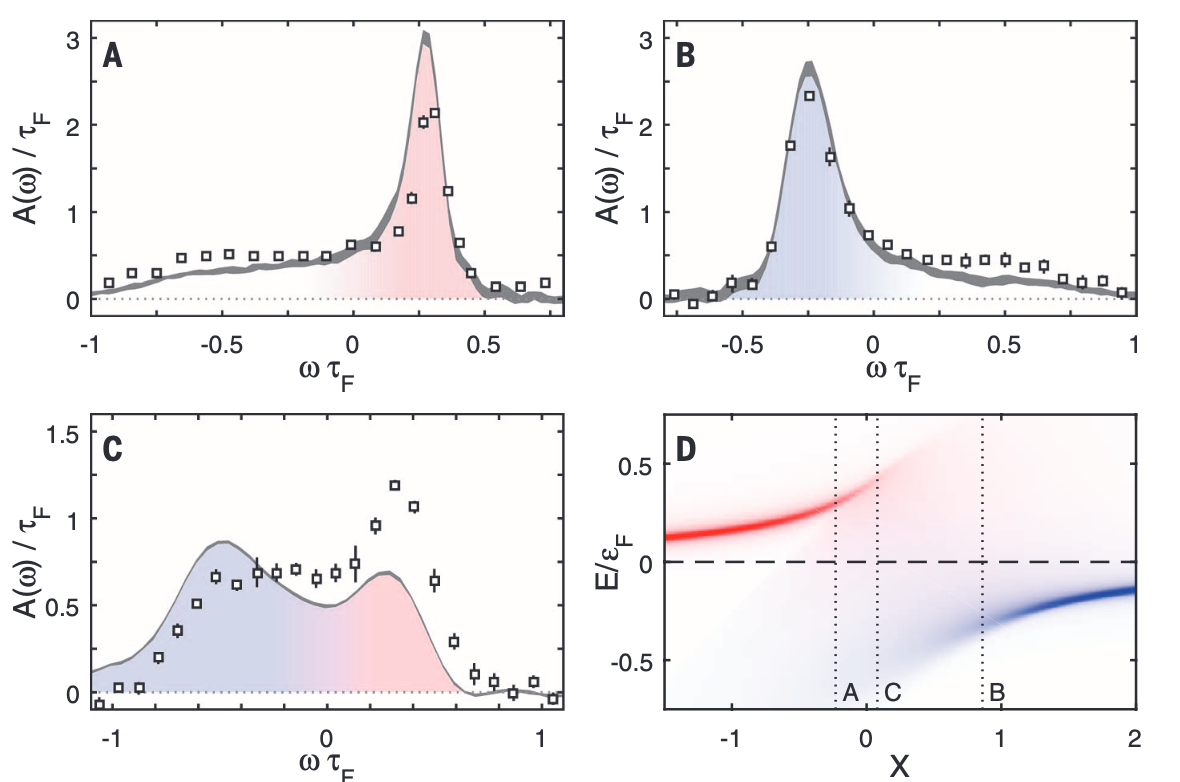
\includegraphics[width=0.7\textwidth]{chap1fpultra.png}
    \bicaption{摘自SU(N) exp}{Reprinted from SU(N) exp}
    \label{fpultra}
\end{figure}

有限温度polaron
\begin{figure}[!htbp]
    \centering
    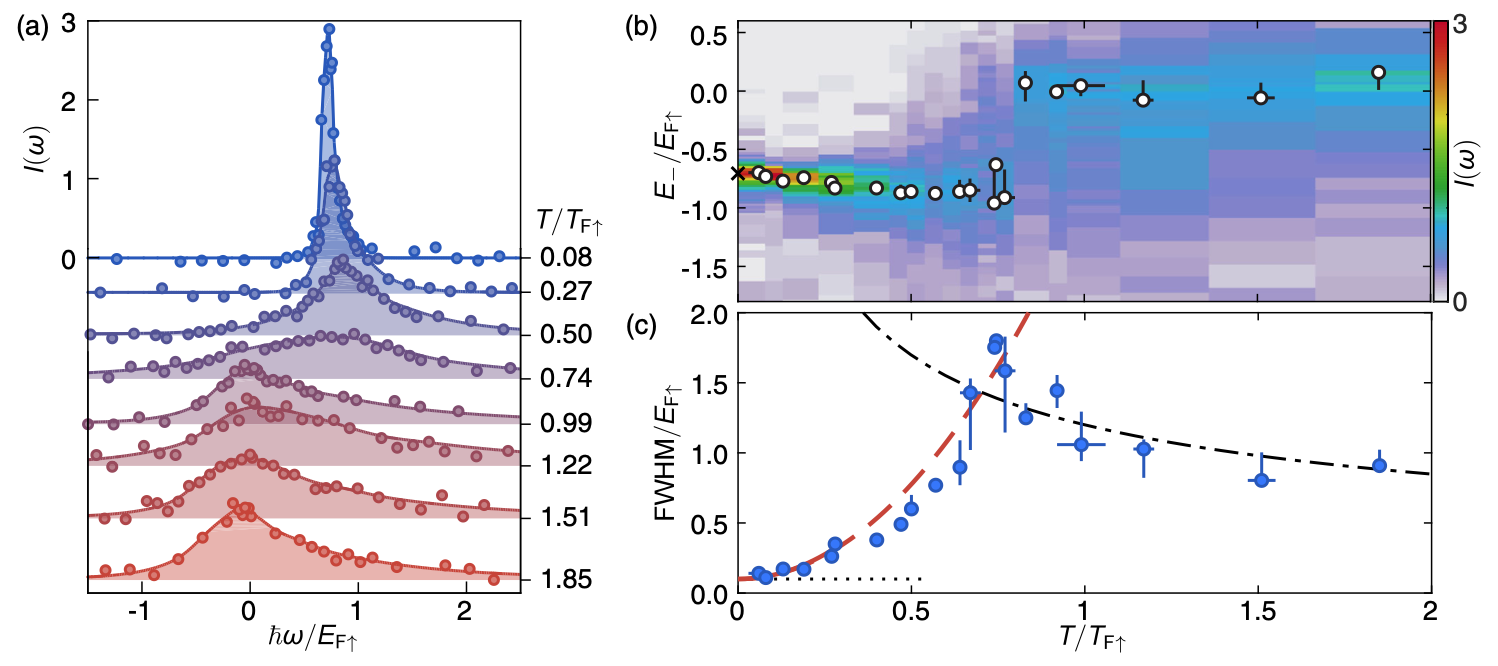
\includegraphics[width=0.7\textwidth]{chap1fpT.png}
    \bicaption{摘自SU(N) exp}{Reprinted from SU(N) exp}
    \label{fpT}
\end{figure}




\subsection{极化子理论}
理论方面关注整个相互作用可调区间,冷原子中费米极化子的研究最早可追溯到Chevy变分波函数,在整个相互作用区间都很好的成立。这是个典型的N+1体系。

1973bishop hard core

chevy2006 V-ph

2007Combescot Feynman Diagram, Massignan P

p-m transition Mora C, Punk M, Combescot R.

MC Pilati S,Prokof’ev N, fix node, diag MC

FRG SchmidtR,

rf spectrum Massignan P

2D, 1D


拓扑极化子

最新进展














